\Chapter{Introduction to Reinforcement Learning}{Definitions and techniques}
\label{ChapterRL} 

% % Intro Chapitre
% The main learning paradigm used throughout this thesis is reinforcement learning. As a machine learning approach and a rich collection of techniques, reinforcement learning greatly influenced the course of this thesis. To understand the context of this thesis, the terminology used, and some of our design choices, we must first introduce the domain of reinforcement learning. In this chapter, we present an overview of this domain and define the learning tools used in the rest of this manuscript. 

% -------------------------------------------------------------------------


\section{Introduction: Definition, Trends and Limitations}\label{sec:RL:Intro}

% Definition
\textbf{Reinforcement Learning} (RL) is a machine learning approach that enables an artificial agent to learn how to act in order to maximise some behaviour-dependent reward signal. The core mechanic of RL is trial-and-error, where the learner sequentially tries actions, obtains rewards, and updates their strategy based on their findings. Throughout many of these cycles, the learner progressively acquires knowledge about the task and devises a strategy to solve it. In this regard, it differs from other machine learning paradigms, namely \textit{supervised} and \textit{unsupervised} learning, that use some fixed set of data points and learn to optimise some objective over this data. With RL, there is no data beforehand, only some definition of the learning environment and the learning agent\footnote{Some forms of RL, like \textit{offline RL}, use previously gathered data to learn RL objectives, but generally this is not the case.}. From there, the agent will generate its own training data by acting in the environment, which will then influence its learning journey. 

% Learning objective
Another key difference is in the optimised objective. In supervised and unsupervised learning, the learning task is defined with some mathematical cost function computed over the model's prediction and the data points. This cost function is usually defined to be easily differentiable so that the model can find a way to minimise it using gradient descent. In RL, the learning task is defined solely by the rewards, that should be maximised. While we will often refer to the reward as a function, in practice it is not a mathematical function of the learner's actions. The reward is a signal given by the environment to the agent: it may be the score in a video game, a note given by a human observer, or a win state (e.g., 1 for "game won", -1 for "game lost", and 0 for "unfinished game") in a tabletop game. Thus, RL algorithms use a series of mathematical tricks to translate the objective of "maximising the rewards" into a learnable objective. This makes learning significantly more difficult. In practice, supervised learning is always preferred to RL if the context allows it. But, it also opens a whole range of possibilities where a learning algorithm can try to optimise any given numerical signal. 

% Learning through reinforcement
A particularly appealing aspect of RL lies in its way of emulating how humans and other animals learn in the real world. In fact, while the term "reinforcement learning" now refers widely to a class of learning algorithms, the idea of learning through reinforcement is also used beyond the scope of computer science. Many concepts of RL derive from neuroscience and are still used to describe the functioning of our brain~\citep{Schultz1997_Neuro, Friston2010_FreeEnergy} or to study mental illness~\citep{Montague2012_Psych}. Reinforcement experiments are used in biology and psychology to characterise intelligence and investigate how learning occurs in animals~\citep{Rescorla1972_Pavlovian, Gardner1984_Chimpanzee, Brembs2010_FreeWill}. RL is also closely tied to evolutionary biology, where evolution can be defined as finding the best strategy to adapt to the environment through natural selection. This definition translates to a whole subclass of RL, suitably called "Evolutionary Algorithms"~\citep{Eiben2003_Evo}. 

% RL in computer science
Coming back to computer science, RL was introduced during the second half of the 20th century, from various fields of research in neuroscience, optimisation, control theory, and electrical engineering~\citep{Sutton2018_RL}. Two main threads can be recognised as direct origins of RL theories. One stems from the ethologist study of learning by trial-and-error, and especially with reinforcing events~\citep{Thorndike1911_AnimalIntell, Rescorla1972_Pavlovian}. These ideas influenced early works in artificial intelligence, later integrating trial-and-error learning into electrical engineering~\citep{Walter1950_MechTortoise} and computer science~\citep{Minsky1961}. The second branch is \textit{dynamic programming}~\citep{Bellman1966_DP}, which investigated solving a complex problem by breaking it into easier sub-problems. This involved the definition of many mathematical tools that became the foundations of RL algorithms (see Section~\ref{sec:RL:Elements}).

% Games for RL
Throughout these developments, various types of problems were studied, starting from recreational games like checkers (see Figure \hyperref[fig:rl-envs]{2.1.a}; \cite{Samuel1959_Checkers}) and tic-tac-toe~\citep{Michie1968_Boxes}. Such games offer a convenient setting for reinforcement learning: the rules and actions are well-defined, the reward function is easy to define (e.g., 1 if the game is won, 0 otherwise), and they are simple enough to be simulated on computers. This last point is crucial, as RL usually requires a large number of experiences to find the optimal strategy, a problem referred to as "\textit{sample inefficiency}". Being able to run fast experiments on simulated environments is critical. With more powerful computers, increasingly difficult games have been tackled with RL methods. Notable instances are TD-Gammon for backgammon~\citep{Tesauro1994_TDGammon} and AlphaGo (see Figure \hyperref[fig:rl-envs]{2.1.f}; \cite{Silver2016_AlphaGo}) which demonstrated how RL techniques could be used to achieve superhuman performance in the challenging game of Go. Following tabletop games, video games have recently been used as playgrounds for RL research. They offer similar advantages (i.e., simulated, scores as rewards) while providing increased complexity in the variety of tasks and environments. The Atari benchmark (see Figure \hyperref[fig:rl-envs]{2.1.e}; \cite{Bellemare2013_Atari}) has been broadly adopted for its wide range of different games that agents play by looking at the pixel images, just like humans do. Recently, the popular video game Minecraft has been invested as a new challenge for artificial intelligence research, thanks to its extremely diverse environment and vast set of acquirable skills (see Figure \hyperref[fig:rl-envs]{2.1.h}; \cite{Oh2016_Minecraft,Guss2019_MineRL}), showing the great potential of modern video games for artificial intelligence research. 

% RL envs
\begin{figure}
\centering
% Gradient Info
\tikzset {_v5yipgm4o/.code = {\pgfsetadditionalshadetransform{ \pgftransformshift{\pgfpoint{0 bp } { 0 bp }  }  \pgftransformrotate{-90 }  \pgftransformscale{2 }  }}}
\pgfdeclarehorizontalshading{_85zdvdaeq}{150bp}{rgb(0bp)=(0.82,0.82,0.82);
rgb(37.5bp)=(0.82,0.82,0.82);
rgb(62.5bp)=(0,0,0);
rgb(100bp)=(0,0,0)}
\tikzset{_9u20o91qg/.code = {\pgfsetadditionalshadetransform{\pgftransformshift{\pgfpoint{0 bp } { 0 bp }  }  \pgftransformrotate{-90 }  \pgftransformscale{2 } }}}
\pgfdeclarehorizontalshading{_vobrdoom8} {150bp} {color(0bp)=(transparent!0);
color(37.5bp)=(transparent!0);
color(62.5bp)=(transparent!10);
color(100bp)=(transparent!10) } 
\pgfdeclarefading{_g2sc87jho}{\tikz \fill[shading=_vobrdoom8,_9u20o91qg] (0,0) rectangle (50bp,50bp); } 
\tikzset{every picture/.style={line width=0.75pt}} %set default line width to 0.75pt        

\begin{tikzpicture}[x=0.75pt,y=0.75pt,yscale=-1,xscale=1]
%uncomment if require: \path (0,935); %set diagram left start at 0, and has height of 935
%Chevron Arrow [id:dp7658333139603358] 
\draw  [draw opacity=0][shading=_85zdvdaeq,_v5yipgm4o,path fading= _g2sc87jho ,fading transform={xshift=2}][line width=0.75]  (16,24.2) -- (16,855) -- (7.9,865) -- (-0.2,855) -- (-0.2,24.2) -- (7.9,34.2) -- cycle ;
%Image [id:dp41541323471887515] 
\draw (150.9,232.79) node  {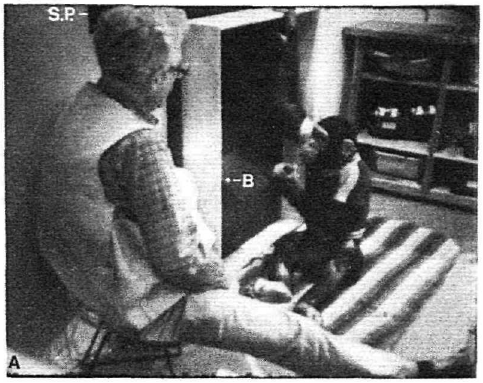
\includegraphics[width=103.65pt,height=82.19pt]{Figures/RL/gardner.png}};
%Image [id:dp007594076672443273] 
\draw (149.8,78.83) node  {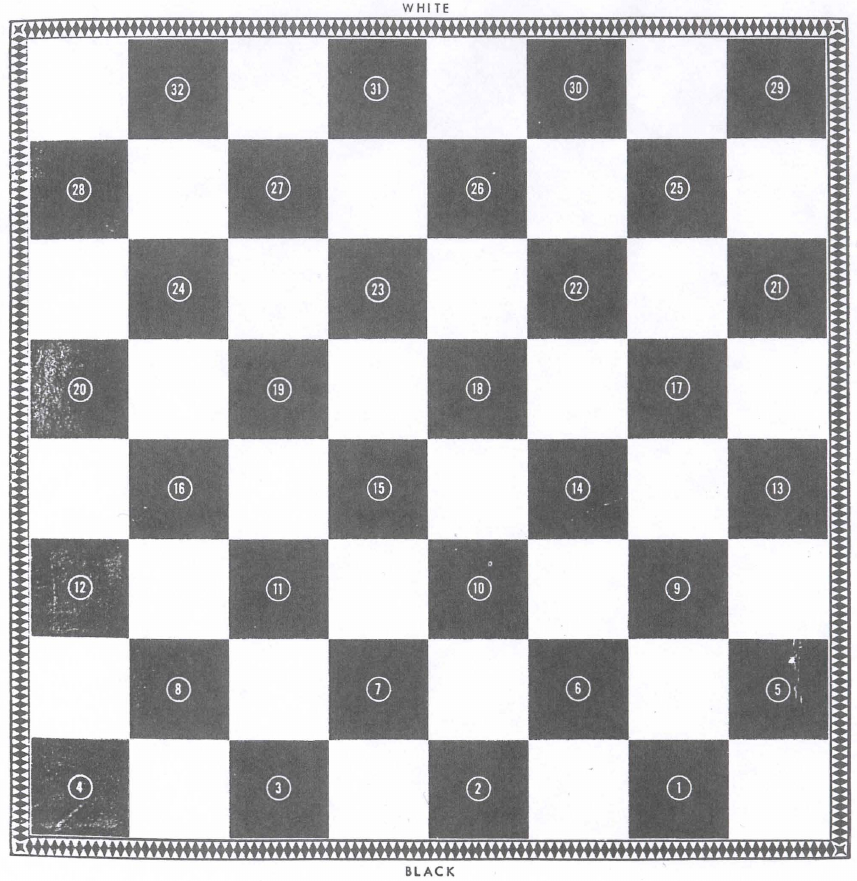
\includegraphics[width=66pt,height=67.85pt]{Figures/RL/checkerSamuel1959.png}};
%Image [id:dp3973383019437343] 
\draw (403.5,102.62) node  {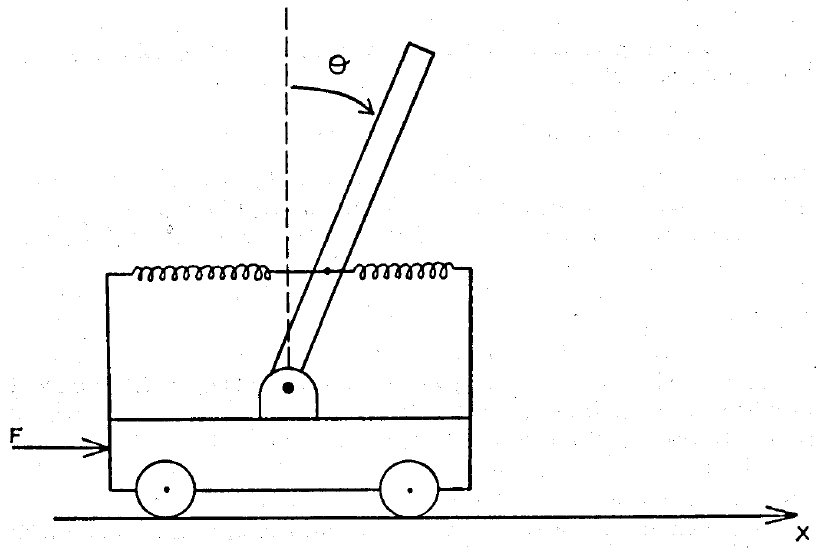
\includegraphics[width=107.25pt,height=72.03pt]{Figures/RL/Michie1968_cartpole.png}};
%Image [id:dp9659625193433798] 
\draw (403.9,257.9) node  {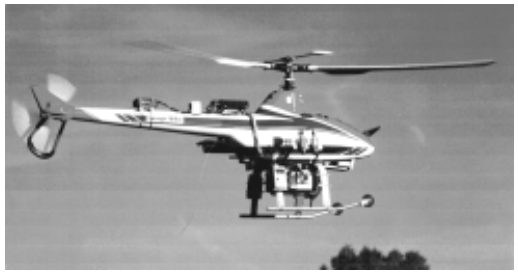
\includegraphics[width=110.25pt,height=63.15pt]{Figures/RL/Bagnell2001-helicopter.png}};
%Image [id:dp976485386281107] 
\draw (400.9,421.92) node  {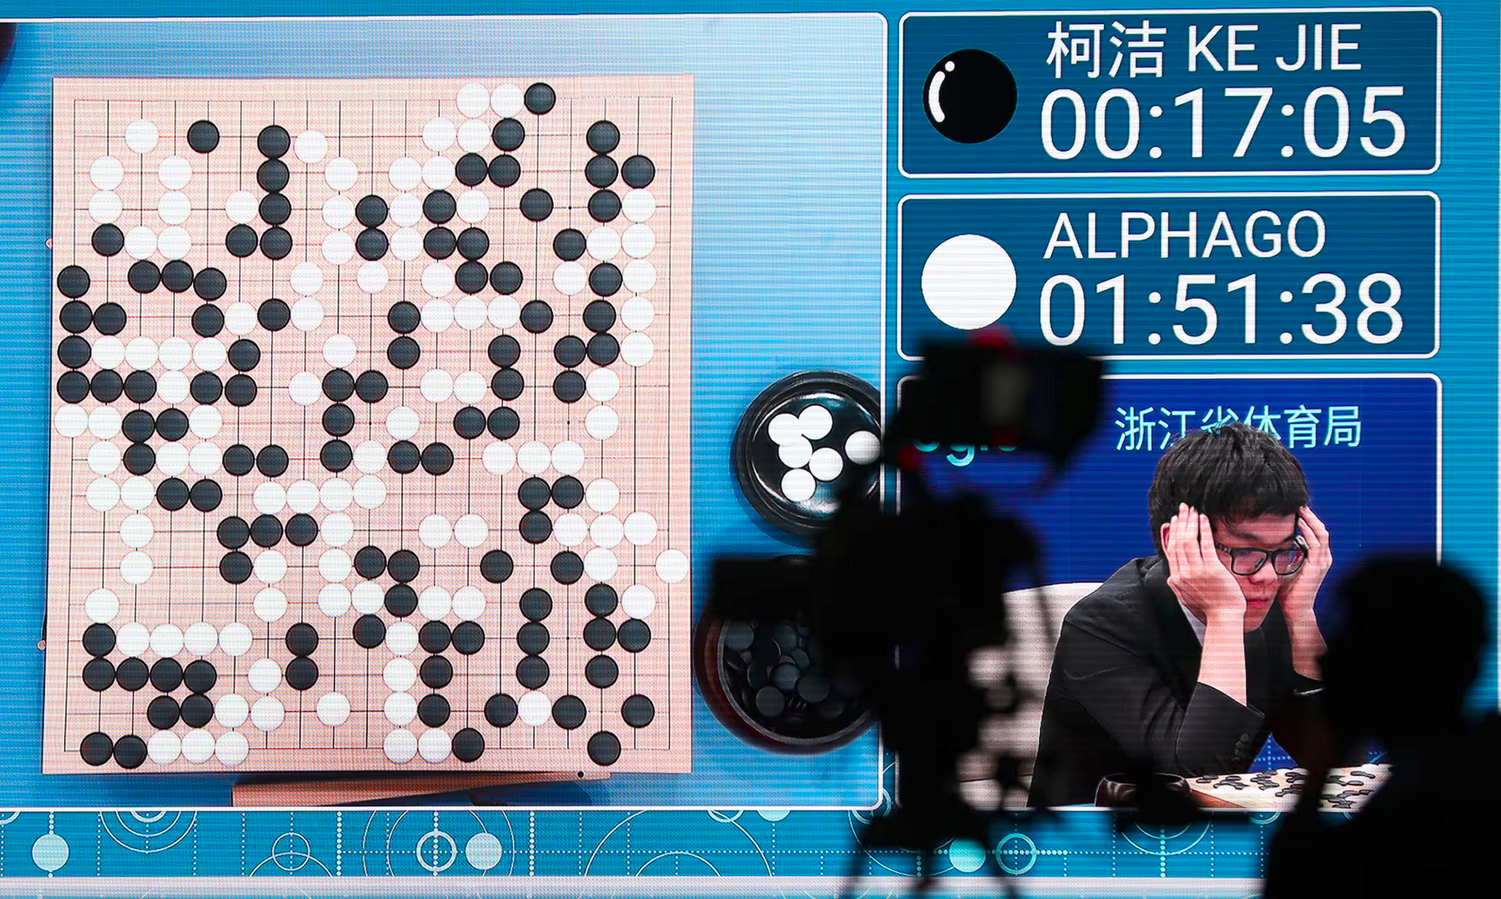
\includegraphics[width=136.05pt,height=81.48pt]{Figures/RL/alphago.png}};
%Image [id:dp6608675188149606] 
\draw (150.5,400.5) node  {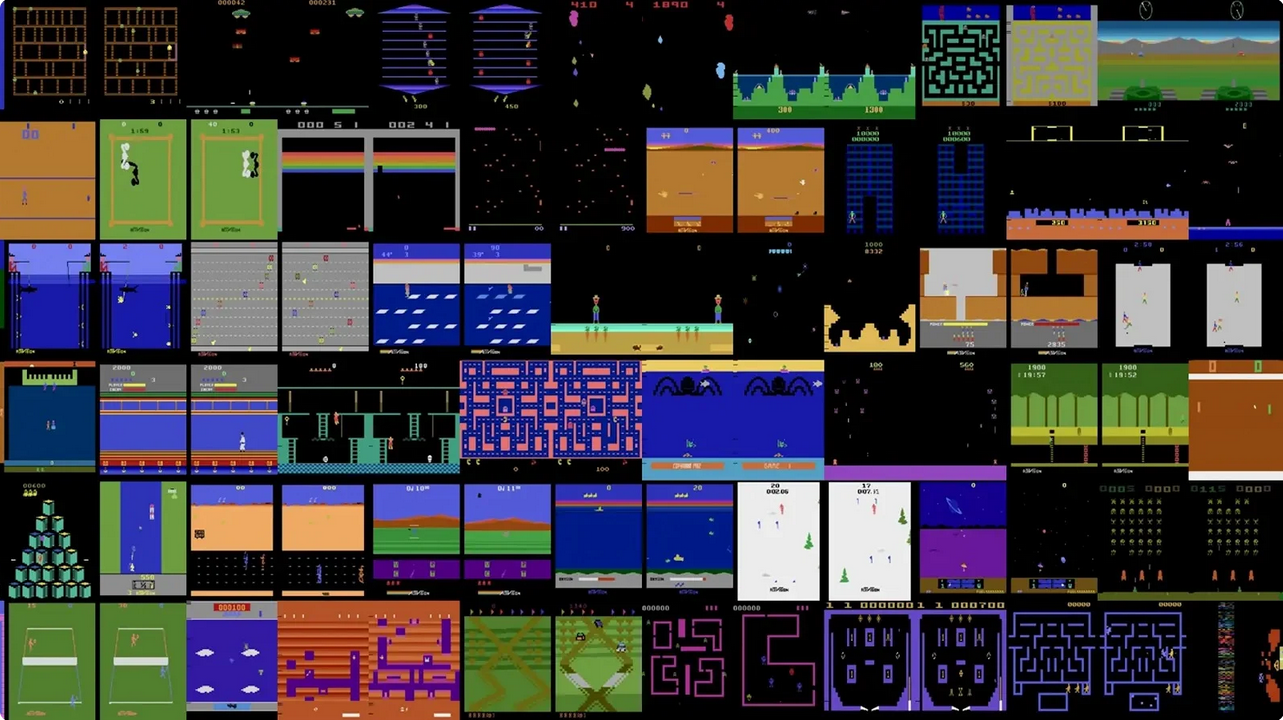
\includegraphics[width=96.45pt,height=87.45pt]{Figures/RL/atari.png}};
%Image [id:dp6327629891315109] 
\draw (149.8,570.8) node  {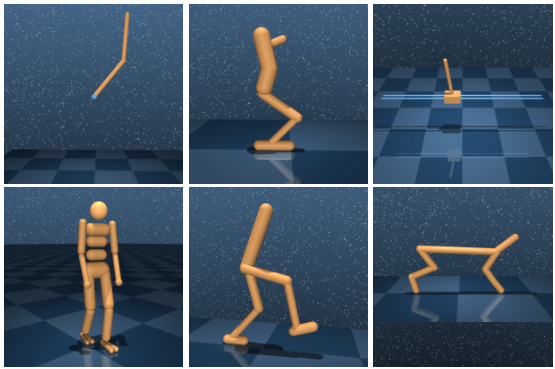
\includegraphics[width=140.7pt,height=91.2pt]{Figures/RL/deepmindcontrolsuite.png}};
%Image [id:dp4430575766949546] 
\draw (397,672.9) node  {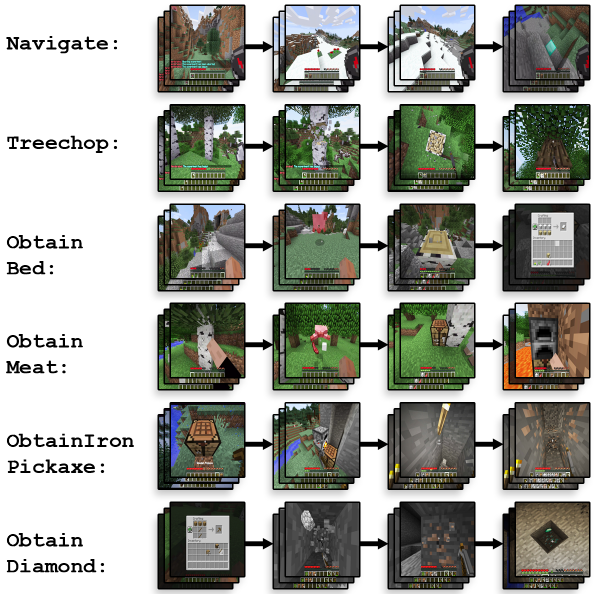
\includegraphics[width=156pt,height=159.15pt]{Figures/RL/minecraft-tasks.png}};
%Image [id:dp21646972126438868] 
\draw (150.7,755.97) node  {
\includegraphics[width=159.45pt,height=89.36pt]{Figures/RL/chatgpt.png}};

% Text Node
\draw (55,291.2) node [anchor=north west][inner sep=0.75pt]  [font=\footnotesize] [align=left] {\begin{minipage}[lt]{140.34pt}\setlength\topsep{0pt}
\begin{center}
{\footnotesize (c) Teaching word to a chimpazee\\ \citep{Gardner1984_Chimpanzee}}
\end{center}
\end{minipage}};
% Text Node
\draw (67.6,126.8) node [anchor=north west][inner sep=0.75pt]  [font=\footnotesize] [align=left] {\begin{minipage}[lt]{114.1pt}\setlength\topsep{0pt}
\begin{center}
{\footnotesize (a) Checkers\\ \citep{Samuel1959_Checkers}}
\end{center}
\end{minipage}};
% Text Node
\draw (325.6,153.2) node [anchor=north west][inner sep=0.75pt]  [font=\footnotesize] [align=left] {\begin{minipage}[lt]{120pt}\setlength\topsep{0pt}
\begin{center}
{\footnotesize (b) Pole-balancing problem\\ \citep{Michie1968_Boxes}}
\end{center}
\end{minipage}};
% Text Node
\draw (316.8,303) node [anchor=north west][inner sep=0.75pt]  [font=\footnotesize] [align=left] {\begin{minipage}[lt]{125.74pt}\setlength\topsep{0pt}
\begin{center}
{\footnotesize (d) Flying an helicopter\\ \citep{Bagnell2001_Helicopter}}
\end{center}
\end{minipage}};
% Text Node
\draw (320.6,480.6) node [anchor=north west][inner sep=0.75pt]  [font=\footnotesize] [align=left] {\begin{minipage}[lt]{113.28pt}\setlength\topsep{0pt}
\begin{center}
{\footnotesize (f) AlphaGo vs. best human \\ \citep{Silver2016_AlphaGo}}\\{\scriptsize (Photograph by Wu Hong, in The Guardian)}
\end{center}
\end{minipage}};
% Text Node
\draw (74.8,464.2) node [anchor=north west][inner sep=0.75pt]  [font=\footnotesize] [align=left] {\begin{minipage}[lt]{106.35pt}\setlength\topsep{0pt}
\begin{center}
{\footnotesize (e) Atari benchmark\\ \citep{Bellemare2013_Atari}}
\end{center}
\end{minipage}};
% Text Node
\draw (32,636.8) node [anchor=north west][inner sep=0.75pt]  [font=\footnotesize] [align=left] {\begin{minipage}[lt]{170.5pt}\setlength\topsep{0pt}
\begin{center}
{\footnotesize (g) Deepmind Control Suite in MuJoCo\\ \citep{Tassa2018_DeepmindControl}}
\end{center}
\end{minipage}};
% Text Node
\draw (300,787.2) node [anchor=north west][inner sep=0.75pt]  [font=\footnotesize] [align=left] {\begin{minipage}[lt]{140.64pt}\setlength\topsep{0pt}
\begin{center}
{\footnotesize (h) Learning skills in Minecraft\\ \citep{Guss2019_MineRL}}
\end{center}
\end{minipage}};
% Text Node
\draw (61.2,823.2) node [anchor=north west][inner sep=0.75pt]  [font=\footnotesize] [align=left] {\begin{minipage}[lt]{123.08pt}\setlength\topsep{0pt}
\begin{center}
{\footnotesize (i) ChatGPT (chat.openai.com)\\ \citep{Ouyang2022_InstructGPT}}
\end{center}
\end{minipage}};
\end{tikzpicture}
\caption{Reinforcement learning environments in various domains of research.}
\label{fig:rl-envs}
\end{figure}

% RL in Robotics
Concurrently to games, RL has also been employed in optimal control and robotics. An early example of this is the classical pole-balancing problem~\citep{Michie1968_Boxes} that features a pole balancing on a moving cart (see Figure \hyperref[fig:rl-envs]{2.1.h}): the cart can move right or left and the reward is made only of a failure signal when the pole falls or the cart reaches the end of the track. While controlling robots is a major drive of RL research, it remains a great challenge. Robotics problems feature high-dimensional, continuous states and actions, which contrast with the discrete, finite states and actions of tabletop games. To overcome this, solutions include partitioning the space of states or actions to reduce complexity using linear function approximation~\citep{Busoniu2017_FuncApprox}, or using neural networks to learn to extract features from continuous states automatically~\citep{Bishop2006_Pattern} (see Section~\ref{sec:NN:DeepLearning}). Another attribute of robotic environments is partial observability, where robots only have incomplete information about the current state of the environment. This has been tackled by learning a model of the dynamics of the environment~\citep{Bagnell2001_Helicopter} (see Section \ref{sec:RL:Model-based}) or by providing the learner with memory to keep track of past information~\citep{Wierstra2007_POMDPs}. Another challenge is the design of a reward function. This requires translating the robot's objective into a numerical signal, which can be tedious. Intuitively, a robot could be rewarded positively when it completes its task. But this kind of sparse reward is difficult to learn. To fix this, reward shaping methods~\citep{Ng1999_Shaping, Laud2004_Shaping} construct rewards to consistently guide the learner towards the objective in a limited number of experiences. Finally, a last great challenge for learning robotic control with RL is the cost of experimenting with robots. Sample inefficiency and learning by trial-and-error make experimenting with physical hardware expensive and time-consuming. For these reasons, some approaches start by learning from demonstrations, before training with RL methods~\citep{Abbeel2006_Helicopter,Vecerik2017_Demonstrations}. Learning from demonstrated sequences of actions simplifies the learning problem by recasting it as a supervised learning problem. Another solution is to turn to simulated environments like ROS~\citep{Macenski2022_ROS} or MuJoCo (see Figure \hyperref[fig:rl-envs]{2.1.g}; \cite{Todorov2012_Mujoco}). However, using a model learnt in simulation in the real world is proven to be a difficult task because of the inevitable gap between the best simulations we have and the real world, a problem termed the "\textit{reality gap}" (see Section~\ref{sec:MAL:RealityGap} for more details on this issue). 
% To bridge this gap, many works have proposed ways to modify the simulated training phase by randomising the parameters of the simulation~\citep{Tobin2017_RealityGap, Chebotar2019_Sim2Real, Andrychowicz2020_Sim2Real} or by learning to efficiently adapt to a different environment~\citep{James2019_Sim2Real}. 
% Ajouter une phrase sur travaux récents qui utilisent rl among other things pour interagir avec des robots (peut-être parler de trucs hierarchiques, Levine2016EndtoEnd)

% RLHF
While control has been a main focus of RL, it has also been studied in other domains of artificial intelligence research. 
% A wide area of RL research has tackled problems in computational economics~\citep{Arthur1991_Economics,Charpentier2021_Economics}. 
A recent success has been the use of Reinforcement Learning from Human Feedback (RLHF;~\cite{Christiano2017_RLHF,Stiennon2020}) in language modelling. Language modelling is the task of learning to predict the next word in a given sequence. In this context, RLHF re-trains initially supervised language models to better fit human preferences. This technique is made possible by using reward modelling~\citep{Leike2018_RewardModel}, where a model learns to predict the rewards given by humans and is then used to train the RL model on a large number of experiences. This allowed the development of conversational agents like the now widely used ChatGPT~\citep{Ouyang2022_InstructGPT}. The success of RLHF approaches demonstrates the great potential of RL for learning to fit human needs. 

% Perspectives and limitations
All these examples show the tremendous potential of RL to shape artificial intelligence research further. This is largely due to the advent of deep reinforcement learning that sparked an ongoing revolution in the field during the last decade. Today, RL is widely considered an important block to building more advanced forms of artificial intelligence, if not the main tool to do so~\citep{Silver2021_RewardEnough}. However, this view is not shared by all~\citep{Mitchell2021_Harder} and RL still suffers from many limitations. We have already mentioned the problems of sample inefficiency, safety, and the high cost of RL training. They all generally hinder performance and prevent RL algorithms from being used extensively in robotics~\citep{Sunderhauf2018_Limits, Ibarz2021_Howto} and autonomous driving~\citep{Kiran2022_DRLDriving, Chen2023_EndToEndDriving}, with supervised alternatives like imitation learning being far superior~\citep{Hester2018_DQNfDemo}. These issues motivate various practical solutions~\citep{Ibarz2021_Howto}, like the aforementioned reward shaping strategy~\citep{Laud2004_Shaping}, as well as whole lines of research such as safe RL that explicitly constrain RL to learn from safe states~\citep{Garcia2015_SafeRL}, and curriculum learning that focuses on designing a schedule of increasingly difficult setups~\citep{Bengio2009_Curriculum, Uchendu2022_Jump}. RL also suffers from more practical issues inherent to its definitions and the tools it uses: reproducibility, high variance, and intricacy of the algorithms and their implementations~\citep{Hendersion2018_Matters}. Finally, as with the rest of methods based on deep neural networks, there is an issue of explainability and interpretability of deep RL. Deep neural networks act as black boxes that have no explicit mean for interpreting their reasoning and, thus, explaining their results~\citep{Rudin2019_StopExplain, Samek2021_ExplainDNN}. With deep RL agents, interpreting the learnt behaviours and understanding how training shaped them this way is often difficult. 
Some solutions are pursued, like hierarchical RL~\citep{Shu2018_Hierarchical, Pateria2021_HRLSurvey, Hafner2022_Hierarchical} or language-augmented RL (see Section \ref{sec:LAMAC:RW_LARL} for a more in-depth review of the literature on this matter).
% Parler de life-long learning/continual RL ?



% -------------------------------------------------------------------------


\section{Elements of Reinforcement Learning}\label{sec:RL:Elements}

\begin{figure}[h]
    \centering
    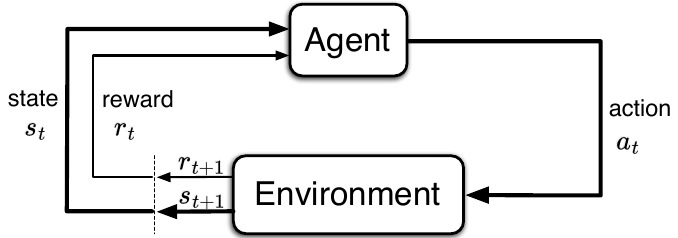
\includegraphics[width=0.8\textwidth]{Figures/RL/rl.jpg}
    \caption{Diagram of the reinforcement learning interaction between the agent and its environment, from \cite{Sutton2018_RL}.}
    \label{fig:rl}
\end{figure}

% Definition of main RL terms
Reinforcement learning is the process of learning how to complete a particular \textbf{task} from trial-and-error. In this process, we refer to the learner as an \textbf{agent}. The agent interacts with its \textbf{environment} over a sequence of discrete time steps denoted by $t=\{0,1,2,...\}$. Each interaction consists in the agent receiving information on its \textbf{state} $s_t$ from the environment and consequently choosing an \textbf{action} $a_t$ to perform. Following the agent's action, the environment produces a \textbf{reward} $r_{t+1}$ and a new state $s_{t+1}$. This process, illustrated in Figure \ref{fig:rl}, repeats indefinitely or stops after a finite number of steps $T$. In the latter case, we call this finite sequence of steps an \textbf{episode}. In the context of RL, the agent's goal is to pick the right actions to maximise the cumulative rewards in the long run. 

% Illustration of these terms
This terminology serves to describe any possible RL setting. The agent refers to the central entity of the experiment, defined concretely as a computer system. It is often considered "\textit{intelligent}" for being: (i) \textbf{reactive} to its environment, perceiving information from its surroundings and acting in response to these input signals; (ii) \textbf{proactive}, shaping its behaviour to satisfy its current goal; (iii) able to \textbf{learn} from its experience~\citep{Wooldridge1995_IntelligentAgents}. The goal of the agent is defined primarily by the task. It can be as straightforward as "picking up an object", or be a more abstract objective like "give this person what they need". The environment refers to the setting where this task is conducted, encompassing all elements except for the agent. The frontier between the agent and the environment is not a physical boundary but rather a conceptual one: everything that cannot be changed arbitrarily by the agent is considered part of the environment. For example, sensors, motors and mechanical joints of a robot should be considered as parts of the environment, while the agent in this case is the program controlling the robot. The states and actions depend on the agent's capabilities in the environment. Like the goal, they can take different forms, with various levels of abstraction. For example, the state of a robot could be concrete information about its surroundings coming from its sensors (e.g., camera, lidar, inertial measurement unit), or more symbolic information like the state of being in a particular room or not. Similarly, actions can be as concrete as "turning 4.5 degrees left", or more high-level like "flip the pancake". The RL framework accounts for all these levels of abstraction, allowing its use in many different settings. 




\subsection{Markov Decision Processes}\label{sec:RL:MDPs}

% States and actions
The universally accepted framework for building RL algorithms is the \textbf{Markov Decision Process} (MDP). The MDP is a mathematical formalisation of the RL problem. It defines this problem as a tuple $\langle\mathbf{S},\mathbf{A},\mathcal{T},\mathcal{R}\rangle$. In this tuple, $\mathbf{S}$ represents the set of all possible states in the environment: $\mathbf{S}=\{S_0,S_1,S_2,...\}$. Similarly, $\mathbf{A}$ is the set of all possible actions: $\mathbf{A}=\{A_0,A_1,A_2,...\}$. In the example of Figure \ref{fig:rl-toy}, $\mathbf{S}$ is the set of all eleven possible positions in the grid, numbered from 0 to 10, and $\mathbf{A}$ contains four possible actions: $\mathbf{A}=\{\mathtt{move\_up},\allowbreak\ \mathtt{move\_right},\allowbreak\ \mathtt{move\_down},\allowbreak\ \mathtt{move\_left}\}$. This setup describes the particular case of a \textit{finite} MDP, where the number of possible states and actions are finite. However, an MDP could also allow infinite states and actions if needed. For example, an autonomous driving system could have its state defined as a continuous GPS position and its action as the continuously defined rotation angle to apply to the steering wheel. 

% Transition probability
Next is the \textbf{transition function} $\mathcal{T}$ that defines the probability of transitioning from state $s$ to state $s'$ by taking action $a$:
\begin{equation}\label{eq:TransitionFunc}
    \mathcal{T}(s'\ |\ s,a)\coloneqq \text{Pr}\{s_{t+1}=s'\ |\ s_t=s,a_t=a\}.
\end{equation}
It dictates how the environment changes after performing an action. The transition function translates the robot's move in terms of probability: for example, in the setup of Figure \ref{fig:rl-toy}, $\mathcal{T}(S_1|S_0,\mathtt{move\_right})=1$ and $\mathcal{T}(S_4|S_0,\mathtt{move\_rigth})=0$. These probabilities describe a \textit{deterministic} environment, where a given action performed in a particular state always leads to the same outcome. On the other hand, in \textit{stochastic} environments, an action may have multiple possible outcomes. For example, an action may fail with a probability of 0.01: $\mathcal{T}(S_1|S_0,\mathtt{move\_rigth})=0.99$ and $\mathcal{T}(S_0|S_0,\mathtt{move\_rigth})=0.01$. In this synthetic environment, we control the probability of each transition. However, in more realistic settings, the transition function is unknown.

% Reward function
Finally, the \textbf{reward function} $\mathcal{R}$ is the expected value of the reward obtained during a transition from state $s$ to $s'$ with action $a$:
\begin{align}\label{eq:RewardFunc}
    \mathcal{R}(s,a)&\coloneqq\mathbb{E}[r_{t+1}\ |\ s_t=s,a_t=a]\notag\\
        &=\sum_{s'\in\mathbf{S}}\mathcal{T}(s'\ |\ s,a)r_{t+1}
\end{align}
In Figure \ref{fig:rl-toy}, the reward function is made of two elements: a positive reward signal if the agent reaches the goal and a negative signal for all other states. The former is straightforward: it indicates that the task is complete. The latter penalises the agent for entering any state that is not the terminal state. This kind of penalty is used often to urge the agent to complete the task as fast as possible: the more steps are taken, the larger the accumulated penalty. The reward depicted in Figure \ref{fig:rl-toy} can be described as \textit{sparse} because there are very few positive reward signals to guide the agent towards the objective. In this simple environment, this should not be an issue. But, in more complex settings with a larger number of possible states, sparse rewards can become problematic.

% Environment dynamics
Often, we see the transition probability and reward function brought together in a single function $p$ that defines the \textbf{environment dynamics}, with:
\begin{equation}
    p(s',r\ |\ s,a)\coloneqq \text{Pr}\{s_{t+1}=s',r_{t+1}=r\ |\ s_t=s,a_t=a\},
    \label{eq:EnvDyn}
\end{equation}
which is the probability of being in state $s'\in\mathbf{S}$ and receiving reward $r\in\mathbb{R}$, after performing action $a\in\mathbf{A}$ in state $s\in\mathbf{S}$.

% RL toy environment
\begin{figure}
    \centering
    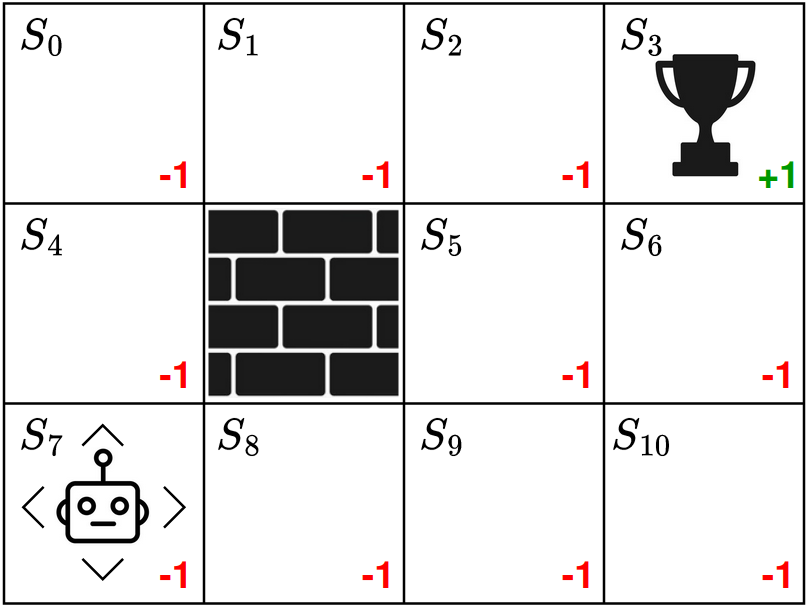
\includegraphics[width=0.5\textwidth]{Figures/RL/rl-toy.png}
    \caption{Simple reinforcement learning environment where the goal is for a robot to navigate in the grid and find the trophy cell. The robot can move in all four directions. The episode ends if the robot reaches the trophy or if the maximum number of steps $T$ is reached. States are defined by the position of the robot in the grid. Rewards for entering each state are indicated in the bottom-right corner of each cell.}
    \label{fig:rl-toy}
\end{figure}





\subsection{Modeling the Agent}\label{sec:RL:Agent}

% Policy
In the context of an MDP, the agent is modelled as a \textbf{policy} that selects actions depending on the current state of the environment. This policy can be either \textit{deterministic} or \textit{stochastic}. A deterministic policy is a function $\pi$ that directly maps the current state $s$ to an action $a$ to perform: $\pi:\mathbf{S}\rightarrow\mathbf{A}$, $\pi(s)=a$. A stochastic policy $\pi$ is defined as a function that maps states to probabilities over possible actions: the probability of choosing each action $a\in\mathbf{A}$ in state $s$ is $\pi(a|s)\in[0,1]$, with $\sum_{a\in\mathbf{A}}\pi(a|s)=1$. The policy function is used to describe how the agent selects its actions. In some algorithms, the policy is explicitly learnt during training. But, the policy might also be arbitrarily based on other learnt elements, or even random or unknown. 

% Trajectory and return
The agent uses the policy function to act in the environment, which results in a sequence of states, actions, and rewards that is called a \textbf{trajectory}, denoted $\tau$:
\begin{equation}
\tau=(s_0,a_0,r_1,s_1,a_1,r_2,s_2,a_2,...).
\end{equation}
The goal of an RL algorithm is to find a policy that maximises the accumulated rewards in the trajectories it generates. To that end, the policy must choose actions to maximise the sum of future rewards which is called the \textbf{return} $G_t$, starting from any step $t$:
\begin{equation}
G_t\coloneqq r_{t+1}+r_{t+2}+r_{t+3}+...+r_T,
\end{equation}
with the episode ending at step $T$. In the case where $T$ is infinite (i.e., the episode never ends) this formulation is problematic as it can result in an infinite return. This motivates another formulation of the return where future rewards are discounted by their distance in time to the current step. This \textbf{discounted return} is defined as:
\begin{equation}\label{eq:return}
    G_t\coloneqq r_{t+1}+\gamma r_{t+2}+\gamma^2 r_{t+3}+...=\sum_{k=0}^{\infty}\gamma^k r_{t+k+1},
\end{equation}
with $\gamma\in[0,1]$ the \textit{discount factor}. The discounted return favours rewards that are closer in time. The value of the discount factor controls how far in time the reward should affect the decision of the agent: a $\gamma$ close to zero will favour immediate rewards, while a $\gamma$ close to one will give importance to long-term returns. In practice, almost all RL methods use the discounted return, even if the episode ends in a finite number of steps $T$. 

% Value function
As the return cannot be computed before the end of the episode, many RL algorithms learn \textbf{value functions} to predict the expected return at any point during the episode. Thus, the \textbf{state-value function} associated with policy $\pi$, is defined as the expected return starting from any state $s$ and following policy $\pi$:
\begin{equation}
    V_\pi(s)\coloneqq\mathbb{E}_\pi[G_t\ |\ s_t=s],
    \label{eq:Value-def}
\end{equation}
where $\mathbb{E}_\pi[.]$ is the expected value of any random variable given that the agent always follows the policy $\pi$. Following the value of a particular state, we can also learn the value of performing a particular action in a particular state. This is the \textbf{action-value function} of policy $\pi$, defined as the expected return starting from state $s$, performing action $a$, and then following policy $\pi$:
\begin{equation}
    Q_\pi(s,a)\coloneqq\mathbb{E}_\pi[G_t\ |\ s_t=s,a_t=a].
    \label{eq:Qvalue-def}
\end{equation}
As we will see in further sections, these value functions can be learnt from experience and then used to choose actions accordingly or to do planning over multiple time steps. 

% Successiveness
An important property of the discounted return defined in Equation~\ref{eq:return} is its successiveness: the return at step $t$ can be expressed in function of the return of the following steps:
\begin{align}
    G_t&\coloneqq r_{t+1}+\gamma r_{t+2}+\gamma^2 r_{t+3}+\gamma^3 r_{t+4}+...\notag\\
       &=r_{t+1}+\gamma(r_{t+2}+\gamma r_{t+3}+\gamma^2r_{t+4}+...\notag\\
       &=r_{t+1}+\gamma G_{t+1}.
\end{align}
The same property can therefore be found for the state-value function:
\begin{align}
    V_\pi(s)&\coloneqq\mathbb{E}_\pi[G_t\ |\ s_t=s]\notag\\
       &=\mathbb{E}_\pi[r_{t+1}+\gamma G_{t+1}\ |\ s_t=s]\notag\\
       &=\mathbb{E}_\pi[r_{t+1}+\gamma V_\pi(s')\ |\ s_t=s,s_{t+1}=s'].
\end{align}

% Optimality
The \textit{optimal policy} is defined as the policy whose expected return is greater than or equal to that of all other possible policies, for all possible states. In other words, a policy $\pi$ is the optimal policy if $V_\pi(s)\geq V_{\pi'}(s)$, for all $s\in\mathbf{S}$ and all possible other policies $\pi'$. The optimal policy, denoted $\pi^*$ is associated with the optimal value functions $V^*$ and $Q^*$. By definition, the optimal policy always chooses the action with the largest action-value. That is,
\begin{equation}
    \pi^*(s)=\argmax_{a\in\mathbf{A}}Q^*(s,a).
\end{equation}
Following this, the optimal state-value function of any state $s$ is equal to the maximum value of $Q^*$ in this state:
\begin{align}
    V^*(s)&=\max_{a\in\mathbf{A}}Q^*(s,a)\notag\\
          &=\max_{a\in\mathbf{A}}\mathbb{E}_{\pi^*}[G_t\ |\ s_t=s,a_t=a]\notag\\
          &=\max_{a\in\mathbf{A}}\mathbb{E}_{\pi^*}[r_{t+1}+\gamma V^*(s')\ |\ s_t=s,a_t=a,s_{t+1}=s'].\label{eq:Bellman-v-exp}
\end{align}
This last result is the \textit{Bellman optimality equation}~\citep{Bellman1957_MDP} for the state-value function. By unfolding the expected value, we get:
\begin{equation}
    V^*(s)=\max_{a\in\mathbf{A}}\sum_{s'\in\mathbf{S}}\mathcal{T}(s'\ |\ s,a)\left[\mathcal{R}(s,a,s')+\gamma V^*(s')\right]. 
    \label{eq:Bellman-v}
\end{equation}
This is another form the Bellman optimality equation that will be used to define RL algorithms in the next section. It can also be expressed for the optimal action-value function as:
\begin{align}
    Q^*(s)&=\mathbb{E}_{\pi^*}[r_{t+1}+\gamma\max_{a'\in\mathbf{A}}Q^*(s_{t+1},a')\ |\ s_t=s,a_t=a]\notag\\
          &=\sum_{s'\in\mathbf{S}}\mathcal{T}(s'\ |\ s,a)\left[\mathcal{R}(s,a,s')+\gamma\max_{a'\in\mathbf{A}}Q^*(s',a')\right]. \label{eq:Bellman-q}
\end{align}
Bellman optimality equations are the basis of most RL algorithms, as they allow to gradually learn the optimal value functions through an iterative process described in Section~\ref{sec:RL:ValueIter}. In finite MDPs, the optimal value functions are proven to exist and be unique. But, that is not the case for more complex environments. Therefore, RL algorithms usually learn to estimate these functions through various techniques. 
%However, in environments with many possible states, this can require tremendous amounts of computational power and memory. The challenge becomes even more apparent in the case of an MDP with a continuous state space, i.e., a infinite number of different states. Thus, the algorithms presented in the next sections are used not necessarily to find the exact optimal behaviour, but rather to approximate the best way possible. Different approaches are developed to make these approximations better and, importantly, to reduce the computational power needed to learn fine policies for the agent. 

% Models
Finally, another tool used in RL is a \textbf{model} of the environment. A model predicts the outcomes of the agent's action in terms of changes in the environment and resulting rewards. Concretely, a model learns to approximate the environment dynamics $p$ defined in Equation~\ref{eq:EnvDyn}. Thus, the model is a function $\widehat{p}$ that maps the current state and action to the next state and reward. It can output a direct prediction, with $\widehat{p}:S\times A\rightarrow S\times\mathbb{R}$, or a probability distribution over states and rewards (like in Equation~\ref{eq:EnvDyn}).
%Similarly to the policy function, it can take two forms depending on the nature of its output. A \textit{distribution model} outputs a probability distribution over all states and rewards, like in Equation (\ref{eq:EnvDyn}). A \textit{sample model} outputs one possible transition based on the current state and action: $\widehat{p}:S\times A\rightarrow S\times\mathbb{R}$. Note that, given a distribution model, we can easily derive a sample model by sampling from the distribution. 
These two forms of models can be used in different ways for doing \textit{planning} over one or multiple time steps. As we will see in Section \ref{sec:RL:Model-based}, planning usually involves looking ahead by predicting future outcomes and then using these predictions to compute or improve value function predictions, which, in turn, can be used to select actions that maximise the expected return. 



% -------------------------------------------------------------------------



\section{Foundational RL Algorithms}\label{sec:RL:Algorithms}

After introducing the core elements used in RL, we present different approaches to learning from reinforcement. These approaches rely on learning value functions, policies, models, or a combination of the three, to devise an efficient strategy of actions. In this section, we present the foundational RL algorithms that serve as a basis for building deep RL and multi-agent RL methods. 


\subsection{Value Estimation}\label{sec:RL:Value-based}

% Introduction
As presented in the last section, value functions are a fundamental component of RL as they aim to predict the most important thing for the agent: the expected return of its actions. In RL algorithms, value functions are used for two different purposes:
\begin{itemize}
    \item First, to evaluate a given policy, which may be unknown, by estimating the expected return obtained following this policy. 
    \item Second, to explicitly learn a strategy to control the agent, in which case the agent's policy will be derived from the learnt value function. 
\end{itemize}
In both cases, the algorithms presented learn estimates of the value functions defined in the last section (see Equations~\ref{eq:Value-def} and~\ref{eq:Qvalue-def}). 


\subsubsection{Value Iteration}\label{sec:RL:ValueIter}

% Value iteration
To learn a value function estimate, a basic technique is \textit{value iteration}. It learns through an iterative process of gathering experience and improving the value function. Value iteration turns the Bellman optimality equations (see Equations \ref{eq:Bellman-v} and \ref{eq:Bellman-q}) into an update rule. That is, given a value function $V$ at our disposal, we compute a new value function based on the result of the Bellman equation:
\begin{equation}
    V(s)\leftarrow\max_{a\in\mathbf{A}}\sum_{s'\in\mathbf{S}}\mathcal{T}(s'\ |\ s,a)\left[\mathcal{R}(s,a,s')+\gamma V(s')\right],
    \label{eq:Value-iter}
\end{equation}
for each state $s\in\mathbf{S}$. The arrow indicates that we replace the current value $V(s)$, typically stored in a table with one value for each state, with a new one resulting from the calculation. In finite MDPs, executing this one time yields a new value function that is necessarily closer to the optimal value function. Thus, starting with an arbitrary initial value function (e.g., $V(s)=0$ for all $s\in\mathbf{S}$), repeating the value iteration operation ensures that $V$ converges towards $V^*$. In Figure \ref{fig:value-iter}, value iteration is executed on the simple RL environment previously introduced. This example shows how value iteration can learn the optimal value function quickly in a simple environment with a limited number of states. 

% Bootstrapping
An interesting property of such algorithms is the fact that they use the current estimate to compute the new one. This is called \textit{bootstrapping}. As we will see, this feature is at the core of many value estimation methods. Bootstrapping can greatly improve the convergence speed of these algorithms: in Figure \ref{fig:value-iter}, using the current estimate $V$ allows each iteration to have more impact (depending on the order in which states are processed). But, this can also induce difficulties: in more complex settings, using imperfect estimates can sometimes produce even worse new estimates, thus compromising the learning process. 

% Illustration of Value iteration
\begin{figure}
    \centering
    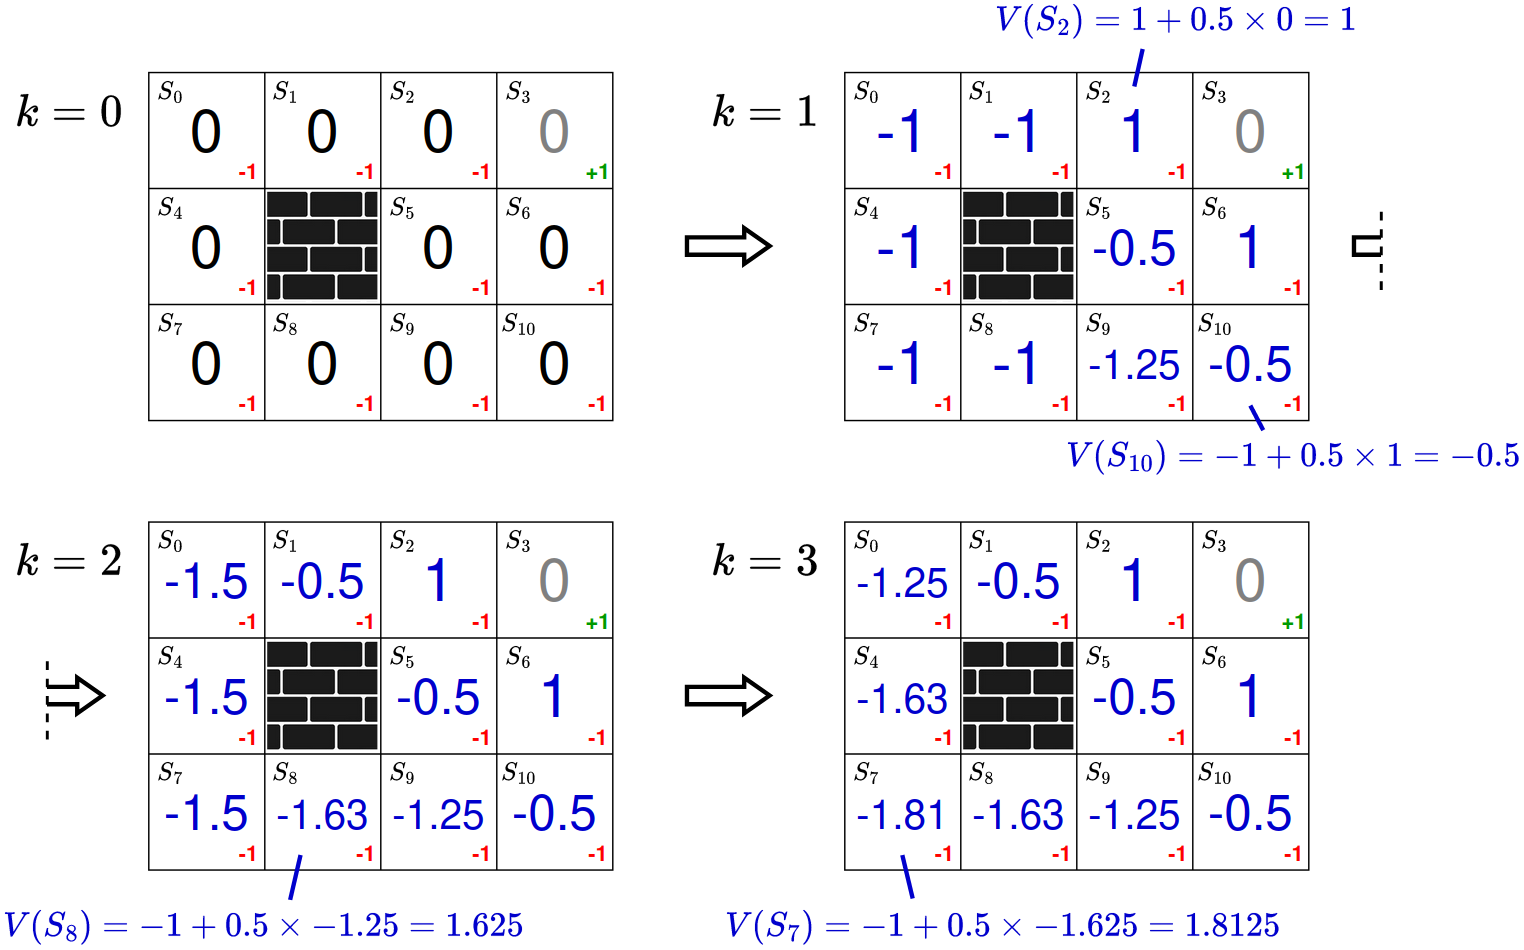
\includegraphics[width=1\linewidth]{Figures/RL/value-iter.png}
    \caption{Value iteration algorithm executed on the example of Figure \ref{fig:rl-toy}. We start with an initial value function $V(s)=0$ for all $s\in\mathbf{S}$. Then, each iteration $k$ applies the update rule of Equation~\ref{eq:Value-iter}, with $\gamma=0.5$, with the result $V(S_t)$ shown in the corresponding cell. As state $S_3$ is terminal, its value is considered to be 0. In three iterations, we converge to the optimal value function. Note that, because we compute the new $V$ for each state successively, the order of the states affects the result of each iteration and the number of iterations required for converging.}
    \label{fig:value-iter}
\end{figure}

\subsubsection{Monte Carlo Methods}\label{sec:RL:MonteCarlo}

% Monte-Carlo
A crucial drawback of the value iteration algorithm is that it assumes complete knowledge of the environment dynamics. Only because we know the probabilities of all transitions and their resulting reward, are we able to compute the expected value in the update rule (\ref{eq:Value-iter}). In most RL settings, the environment dynamics are unknown. Therefore, it is impossible to compute the exact value iteration update rule. What is often possible, however, is to run simulated experiments and gather sequences of states, actions and rewards. This is called "\textit{sampling}" trajectories from the environment. These sampled trajectories can then be used to compute approximations of what we want to predict. For example, given a trajectory $\tau$ generated using the sampling policy $\pi$, we can compute the return from any state $s\in\tau$ (according to Equation~\ref{eq:return}) and use the result as an estimation of the expected return from state $s$, i.e., $V_\pi(s)$. This is the core idea behind \textbf{Monte Carlo} methods: estimating the value function of a given policy by averaging sampled returns. This can be performed iteratively, by keeping a running estimate of the value function and updating it after each episode with:
\begin{equation}
    V_\pi(s_t)\leftarrow V_\pi(s_t)+\alpha\left[G_t-V_\pi(s_t)\right],
    \label{eq:Monte-Carlo}
\end{equation}
for all $t<T$, with $G_t$ the experienced return from state $s_t$ and $\alpha\in]0,1]$ a constant parameter called the \textbf{learning rate}. This update modifies the value of $V_\pi(s_t)$ by "moving it" towards the experienced return. The learning rate $\alpha$ controls the magnitude of this modification: $\alpha=1$ would mean the new value of $V_\pi(s_t)$ is $G_t$, $\alpha<1$ yields a new value between the old $V_\pi(s_t)$ and $G_t$. Using a learning rate is important because one sampled return is a poor approximation of the actual state-value function. Thus, repeating this update many times will allow to gradually move towards a better estimate of $V_\pi(s_t)$.

\subsubsection{Temporal Difference Learning}\label{sec:RL:TD}

% TD
A problem with Monte Carlo methods is that they require waiting for the end of each episode to compute the return of all states. In some environments, the episode might last for several hours or even never end, making Monte Carlo methods impractical. A solution for this is to use \textbf{Temporal-Difference} (TD) learning~\citep{Sutton1988_TD}. TD methods similarly learn an estimate of the value function, but using only a limited number of transitions. The simplest TD method, called \textit{TD(0)}, updates the value after only one time step, with
\begin{equation}
    V_\pi(s_t)\leftarrow V_\pi(s_t)+\alpha\left[r_{t+1}+\gamma V_\pi(s_{t+1})-V(s_t)\right].
    \label{eq:TD}
\end{equation}
The return in the Monte Carlo update rule (Equation~\ref{eq:Monte-Carlo}) is replaced by its estimation using the current value function. The expression inside the brackets is often referred to as the \textit{TD-error} or \textit{Bellman error} as it is derived from the Bellman equation (\ref{eq:Bellman-v}). It measures the difference between the current estimated value of $s$ and the better estimate $r_{t+1}+\gamma V_\pi(s_{t+1})$ given by TD(0), called the \textit{TD-target}. The TD-target, can be extended to use the experience of multiple time steps to have a better estimate of the return~\citep{Sutton1988_TD}. 
%However, the one-step version is often preferred for its simplicity. 

% SARSA
% For now, we have shown how to find the value function associated to a given policy that produces trajectories. We will show in the next sections how this can help learning better policy functions. But, with only a value function, TD applied to the action-value function can learn an effective policy to control the agent. Similarly to Equation~\ref{eq:TD}):
% \begin{equation}
%     Q(s_t,a_t)\leftarrow Q(s_t,a_t)+\alpha\left[r_{t+1}+\gamma Q(s_{t+1},a_{t+1})-Q(s_t,a_t)\right].
%     \label{eq:SARSA}
% \end{equation}
% This update rule uses the tuple $\langle s_t,a_t,r_{t+1},s_{t+1},a_{t+1}\rangle$ to update the current estimate of $Q$. This tuple gave its name the to the algorithm \textit{SARSA}~\citep{} that uses this update rule to learn a better action-value function and use it for control. To do so, the agent simply chooses the action with the highest action-value. After each transition, the action-value function can be updated using the experience of the last two steps. 

\subsubsection{Q-Learning}\label{sec:RL:Qlearning}

% Q-learning
For now, we have looked at methods to learn estimates of the state-value function. The \textit{Q-learning} algorithm~\citep{Watkins1989_RL} applies TD learning to the action-value function to directly learn an efficient way to control the agent. Given many transition tuples of form $\langle s_t,a_t,r_{t+1},s_{t+1}\rangle$, we can learn an action-value function $Q$ with:
\begin{equation}
    Q_\pi(s_t,a_t)\leftarrow Q_\pi(s_t,a_t)+\alpha\left[r_{t+1}+\gamma\max_aQ_\pi(s_{t+1},a)-Q_\pi(s_t,a_t)\right].
    \label{eq:Qlearning}
\end{equation}
This update rule uses the current estimate $Q$ as an approximation of the optimal $Q^*$ to compute the Bellman error. With this update, Q-learning learns the action-value function of the "\textit{greedy} policy with respect to $Q$", i.e., the policy that always chooses the action with the highest action-value according to Q: $\pi(s)=\argmax_aQ_\pi(s,a)$. Given enough training, the learnt action-value function can be used to choose actions following the greedy policy. 

% Exploration-Exploitation
This method is shown to effectively learn a good approximation of $Q^*$ as long as all states are explored enough. Thus, it requires a sampling policy to explore the environment and gather the transition tuples. The simplest possible policy is to randomly select actions in all steps. But, this means that some irrelevant states will be explored as much as others. Instead, we might want to focus on the states and actions that have more potential. This is a common dilemma in RL algorithms, where we need to balance a trade-off between \textit{exploration} and \textit{exploitation}:
\begin{itemize}
    \item We want to explore different behaviours to better understand the environment dynamics and improve our estimations. 
    \item But, at the same time, we want to exploit our past findings to learn faster.
\end{itemize}
In the case of Q-learning, exploration is done by randomly selecting actions. And, exploitation is done by using the greedy policy to select action.  

% Epsilon-greedy
To balance the exploration-exploitation trade-off, Q-learning employs the $\epsilon$\textit{-greedy} policy. At each time step, $\epsilon$-greedy decides between choosing an action randomly or following the greedy policy. It uses a parameter $\epsilon$ between 0 and 1 that determines the probability of choosing the action randomly. Typically, this parameter starts at 1 and decreases throughout training towards 0. This allows a progressive shift between random exploration at the start when the estimations are bad, and exploitation when estimations start getting better. While this is far from being a perfect exploration strategy (more on that in Chapter \ref{ChapterJIM}), it offers a simple solution for exploration in Q-learning. An algorithm for executing Q-learning with $\epsilon$-greedy is described here: 
\begin{algorithm}
\caption{Q-learning with $\epsilon$-greedy policy}
\label{alg:q_learning}
\begin{algorithmic}
\State Initialize $Q(s, a)$ arbitrarily
\State Initialize $\epsilon=1$
\State Initialize $\alpha$ (learning rate), $\gamma$ (discount factor)
\For{each episode}
    \State Initialize state $s_0$
    \For{t=0,...,T}
        \State Execute $\epsilon$-greedy policy:\\
        \hspace{45pt} With probability $\epsilon$, choose a random action $a_t$\\
        \hspace{45pt} Otherwise, choose $a_t = \argmax_a Q(s_t, a)$
        \State Perform action $a_t$, observe reward $r_{t+1}$ and new state $s_{t+1}$
        \State $Q(s_t, a_t) \gets Q(s_t, a_t) + \alpha \left[r_{t+1}+\gamma\max_{a}Q(s_{t+1},a)-Q(s_t,a_t) \right]$
        \State $s_t\gets s_{t+1}$
        \State $\epsilon\gets\text{max}(\epsilon-0.001,0)$
    \EndFor
\EndFor
\end{algorithmic}
\end{algorithm}

% Tabular
An important observation to make about all value-based methods presented in this section is the fact that they all rely on a list of values to keep track of the current estimations. In Q-learning, for example, the action-value function is represented as a table with states as rows and actions as columns, where each cell $(s,a)$ contains the current estimate $Q(s,a)$. For this reason, these approaches are qualified as "tabular". This aspect highlights a clear drawback of these methods: they are limited in the number of single values they can keep track of. To learn a perfect policy or value function, we would need to exhaustively try all possible actions in all possible states. But, this is impossible in rich environments with very large, if not continuous, state and action spaces. Thus, tabular value functions are limited to environments where they can realistically explore all states or state-action pairs enough times to build good value estimates. In fact, they are even incapable of dealing with continuous states and actions, as they would require infinitely large value tables, which makes their application to real world tasks significantly more difficult.

% Parameterised value
A solution for this is to change the form of the value function and represent it as a parameterised function. Instead of keeping track of all values in a table, the value function is defined as a mathematical function of states that outputs the value of the input state. We would write the value functions as $V(s,\varphi):S\times\mathbb{R}^{d^\varphi}\rightarrow\mathbb{R}$ or $Q(s,a,\varphi):S\times A\times\mathbb{R}^{d^\varphi}\rightarrow\mathbb{R}$, with $\varphi\in\mathbb{R}^{d^\varphi}$ a vector of parameters of dimension $d^\varphi$ used to define the value function. The actual definition of the function is arbitrary. It can be as simple as a linear transformation of the input state, or use more complex definitions such as artificial neural networks (see Section \ref{sec:NNs}). In any case, $\varphi$ is the set of real-valued parameters that dictates the outputs of the value function. An advantage of having a parameterised value function is that it can now deal with continuous states. There is no more table keeping track of all possible values. The new value function should now be able to predict the value of states it has never seen before, by generalising from its training experience (see Section~\ref{eq:DQN} for more detail). But, this also comes with downsides. Learning a set of parameters that generalises well can be difficult. From the designer's point of view, the value function is now a black box that computes values from a series of mathematical operations, which can be hard to interpret. 

% Conclusion
Despite their limitations, value-based approaches are still widely used across RL research. Their simple definition and low computational resources make them easy to implement. In the next sections, we will describe ways to alleviate some of the drawbacks of value-based algorithms. Furthermore, we will see that, when combined with other techniques, value functions play a crucial role in building good RL agents. 

\subsubsection{On-Policy vs. Off-Policy Learning}\label{sec:RL:On/Off-policy}

% On- vs Off-policy (SARSA)
Q-learning, as defined in Algorithm \ref{alg:q_learning}, is characterised as an \textbf{off-policy} algorithm, because its update does not depend on the policy used to generate the experience, which is referred to as the \textit{behaviour} policy. This is in contrast with \textbf{on-policy} algorithms, such as SARSA~\citep{Rummery1994_SARSA}, that learns an action-value function, similarly to Q-learning, but based on an experience tuple $\langle s_t,a_t,r_{t+1},s_{t+1},\\a_{t+1}\rangle$:
\begin{equation}
    Q(s_t,a_t)\leftarrow Q(s_t,a_t)+\alpha\left[r_{t+1}+\gamma Q(s_{t+1},a_{t+1})-Q(s_t,a_t)\right].
    \label{eq:SARSA}
\end{equation}
The difference with the Q-learning update (see Equation~\ref{eq:Qlearning}) is in the choice for action at state $s_{t+1}$, used in the TD-target:
\begin{itemize}
    \item SARSA uses the action $a_{t+1}$ that was selected by the behaviour policy. Therefore, its update depends on the current behaviour policy of the agent (i.e., on-policy).
    \item Q-learning uses the learnt action-value to select a greedy action that serves as $a_{t+1}$ in the TD-target: $r_{t+1}+\gamma\max_{a}Q(s_{t+1},a)$. This TD-target depends only on $Q$ and is independent of the behaviour policy (in this case the $\epsilon$-greedy policy). Thus, Q-learning is off-policy. 
\end{itemize}
In other words, off-policy value learning learns the value of a policy (in this case, the greedy policy with respect to $Q$), using another policy to gather experiences (here, $\epsilon$-greedy). On the other hand, on-policy value learning directly learns the value of the behaviour policy. Note that, while we illustrate these properties with action-value learning algorithms, these can be used to characterise state-value or policy learning algorithms (see Sections \ref{sec:RL:Policy-based} and \ref{sec:DRL:Policy}).

% Experience Replay
The distinction between on- and off-policy is subtle but has one major implication. Off-policy algorithms can learn functions (value or policy) based on data generated by other, totally separate processes. For example, Q-learning could learn the optimal action-value function based on experiences gathered by a random policy, a pool of various independent policies, or even human experts. This particular feature allows using \textbf{experience replay}~\citep{Lin1992_ExperienceReplay}, where, during training, experiences are stored in a memory, called the \textit{replay buffer}, and are then reused any number of times in later updates. To make an update, a batch of past experiences is drawn randomly from the replay buffer and the learning update is performed on all these samples. Training on past experiences allows learning on more diverse data, thus specialising less on the current behaviour policy. In this case, off-policy learning is required because the replay buffer is full of past experiences generated by previous (different because trained fewer times) versions of the behaviour policy. 






\subsection{Policy Gradients}\label{sec:RL:Policy-based}

\subsubsection{Learning a Parameterised Policy Function}

% Learning a parameterised policy
In Section \ref{sec:RL:Agent}, we said that an RL agent is primarily defined by its policy function $\pi$, which maps states to actions. We saw in the last section that value functions can be used to evaluate an unknown policy or even to learn a policy by being greedy with respect to an action-value function. Another possible approach is to directly learn the policy function. This can be done by representing the policy function as a parameterised mathematical function of states which outputs either a probability over possible actions, in the case of a stochastic policy, or directly the action to perform, for a deterministic policy. For these two possible cases, we write:
\begin{equation}
    \pi(a\ |\ s,\theta)=Pr\{a_t=a\ |\ s_t=s,\theta_t=\theta\},
\end{equation}
or
\begin{equation}
    \pi(s;\theta)=a,
\end{equation}
where $\theta\in\mathbb{R}^{d^\theta}$ is the set of learnt parameters of the policy function. We also denote such policy $\pi_{\theta}$, as the policy defined by parameters $\theta$. 

% Gradient ascent
To maximise future rewards, we have to find the set of values for $\theta$ that produces the best sequences of actions. To do so, we can sample experiences from the environment and accordingly modify $\theta$ to improve the policy. This can be done using \textbf{gradient ascent}, which gradually modifies the parameters to maximise a given measure of performance $J(\theta)$:
\begin{equation}
    \theta_{t+1}=\theta_t+\alpha\nabla J(\theta_t),
    \label{eq:GradientAscent}
\end{equation}
where $\alpha\in]0,1]$ is a small learning rate and $\nabla J(\theta_t)$ is the gradient of the objective $J(\theta_t)$ with regards to the policy parameters $\theta$ at time step $t$. It is a vector that shows in which direction in the parameter space to move $\theta$ to maximise the objective. Thus, Equation~\ref{eq:GradientAscent} replaces the current parameters $\theta_t$ with a new set of values $\theta_{t+1}$ that yields better values of $J$. 



\subsubsection{The Policy Gradient Theorem}\label{sec:Policy:PolicyGradientTheorem}

% Policy gradient theorem
In RL, the objective to maximise is the sum of future rewards. Thus, we can define the objective using the true value function of our policy: $J(\theta)=V_{\pi_{\theta}}(s_0)$, with $s_0$ being the initial state of the episode. Given this, for a discrete MDP and a given stochastic policy $\pi_{\theta}$, we can devise the \textbf{policy gradient theorem} that yields:
\begin{equation}
    \nabla J(\theta)=\sum_s\rho_{\pi_{\theta}}(s)\sum_aQ_{\pi_{\theta}}(s,a)\nabla\pi_\theta(a\ |\ s),
    \label{eq:PolicyGradient:Theorem}
\end{equation}
with $Q_{\pi_{\theta}}$ the true action-value function of policy $\pi_{\theta}$ and $\rho_{\pi_{\theta}}(s)$ the probability of experiencing state $s$ if we follow policy $\pi_{\theta}$. 
%The proof of this theorem is given in Annex \ref{app:RL:PolicyGradientTheorem}. 

% Reinforce
If policy $\pi_{\theta}$ is followed, then the theorem can be formulated with an expected value:
\begin{align}
    \nabla J(\theta)&=\mathbb{E}_{s\sim\rho_{\pi_{\theta}}}\left[\sum_aQ_{\pi_{\theta}}(s,a)\nabla\pi_\theta(a\ |\ s)\right]\label{eq:PolicyGradient:Exp}\\
    &=\mathbb{E}_{s\sim\rho_{\pi_{\theta}}}\left[\sum_a\pi_\theta(a\ |\ s)Q_{\pi_{\theta}}(s,a)\frac{\nabla\pi_\theta(a\ |\ s)}{\pi_\theta(a\ |\ s)}\right]\notag\\
    &=\mathbb{E}_{s\sim\rho_{\pi_{\theta}},a\sim\pi_{\theta}}\left[Q_{\pi_{\theta}}(s,a)\frac{\nabla\pi_\theta(a\ |\ s)}{\pi_\theta(a\ |\ s)}\right].\label{eq:PolicyGradient:sampleA}
\end{align}
The expected value in Equation~\ref{eq:PolicyGradient:Exp} is obtained by sampling $s\sim\rho_{\pi_{\theta}}$. Likewise, in Equation~\ref{eq:PolicyGradient:sampleA}, the sum is absorbed in the expectation by sampling $a\sim\pi_{\theta}$. Because $Q_{\pi_\theta}(s,a)=\mathbb{E}_\pi[G_{s,a}|s,a]$, by definition, we can rewrite the policy gradient as:
\begin{equation}
    \nabla J(\theta)=\mathbb{E}_{\pi_{\theta}}\left[G_{s,a}\frac{\nabla\pi_\theta(a\ |\ s)}{\pi_\theta(a\ |\ s)}\right].
    \label{eq:REINFORCE}
\end{equation}
This expectation can be approximated by sampling many trajectories. The algorithm REINFORCE~\citep{Williams1992_Reinforce} uses this to update the parameters $\theta$:
\begin{equation}
    \theta_{t+1}\leftarrow\theta_t+\alpha G_t\frac{\nabla\pi_\theta(a_t\ |\ s_t)}{\pi_\theta(a_t\ |\ s_t)},
\end{equation}
for any state $s_t$ and action $a_t$ from which the agent has experienced the return $G_t$. In this update, the gradient of the policy indicates the direction, in parameter space, that most increases the probability of choosing action $a_t$. By taking the product of this gradient with the return $G_t$, this update increases the probability of actions depending on the returns they generate. High positive returns will result in high increases in the corresponding actions, and conversely for negative returns. Then, dividing by the probability of the action ensures that actions that are selected more frequently are not over-estimated by getting more updates of the same magnitude. Therefore, the REINFORCE update conveniently increases the probability of choosing actions that yield good returns and decreases the probability of actions that yield bad ones. 

\subsubsection{The Actor-Critic Architecture}\label{sec:Policy:Actor-Critic}
% Actor-Critics
As it uses the complete return, REINFORCE is a Monte Carlo method for learning a parameterised policy function. Like the Monte Carlo approach presented in the last section, REINFORCE requires waiting for the end of the episode to update the policy. But, again, we can use the principle of TD learning (see Section \ref{sec:RL:TD}) to solve this issue, by replacing the return by its estimation with a value function:
\begin{equation}
    \theta_{t+1}\leftarrow\theta_t+\alpha\left(r_{t+1}+\gamma V(s_{t+1})\right)\frac{\nabla\pi_\theta(a_t\ |\ s_t)}{\pi_\theta(a_t\ |\ s_t)},
\end{equation}
or,
\begin{equation}
    \theta_{t+1}\leftarrow\theta_t+\alpha Q(s_t,a_t)\frac{\nabla\pi_\theta(a_t\ |\ s_t)}{\pi_\theta(a_t\ |\ s_t)},
\end{equation}
where $V$ and $Q$ would be learnt value functions that estimate the true value functions of the current policy $\pi$. This kind of approach is referred to as \textit{actor-critic} methods~\citep{Barto1983_ActorCritic, Sutton1984_ActorCritic}, where the policy is the actor who learns to select action, and the value function is the critic who evaluates the policy's actions. In this case, the value function is used only to guide the learning process of the policy. 
% Si besoin dans la suite: ajouter explication des baseline dans PG et A2C ici

% DPG
In the last section, we introduced parameterised value functions as a way to use value functions with continuous states. However, a parameterised version of Q-learning would still not be able to deal with continuous actions efficiently. That is because finding a greedy policy with respect to a continuous action-value function would be an optimisation problem in itself: finding the global maximum of a given function. But, thanks to an actor-critic architecture, a solution to this issue can be found. By extending the policy gradient theorem defined in Equation~\ref{eq:PolicyGradient:Exp} to continuous actions and a deterministic policy, we can find that
\begin{equation}
    \nabla J(\theta)=\mathbb{E}_{s\sim\rho_{\pi_\theta}}\left[\nabla_{\theta}\pi_\theta(s)\nabla_aQ_\varphi(s,a)\ |\ a=\pi_\theta(s)\right].
    \label{eq:DPG}
\end{equation}
This the \textbf{deterministic policy gradient theorem} (DPG), as defined by \cite{Silver2014_DPG}, which gives the following update for the parameters $\theta$:
\begin{equation}
    \theta_{t+1}\leftarrow\theta_t+\alpha_\theta\nabla_\theta\pi_\theta(s_t)\nabla_aQ_\varphi(s_t,a_t).
    \label{eq:DPG}
\end{equation}
The parameters of the action-value function $\varphi$ are updated as well to minimise the Bellman error:
\begin{align}
    \delta_t&=r_t+\gamma Q_\varphi(s_{t+1},a_{t+1})-Q_\varphi(s_t,a_t)\\
    \varphi_{t+1}&\leftarrow\varphi_t+\alpha_\varphi\delta_t\nabla_\varphi Q_\varphi(s_t,a_t).
\end{align}
Intuitively, DPG can be understood as an extension of Q-learning for continuous actions, where the $\epsilon$-greedy policy is replaced by a learnt policy trained to select the actions that maximise $Q_\varphi$. 

% ? Continuous actions (sampling actions)


% Conclusion: policy-based, why, other approaches derived from PG, complementary with values 
All RL approaches that derive from the policy gradient theorem are referred to as \textit{policy-based}, even the actor-critic that also learns value functions. A first appeal to policy-based methods is intuitive: it seems logical to explicitly learn to perform actions more often if they produce better returns, and conversely. The great advantage of policy-based methods, however, is in their capacity to handle continuous state and action spaces~\citep{Williams1992_Reinforce}. Parameterised value functions can deal with continuous states but, as we have seen, are still unable to handle continuous actions without being paired with a learnt policy or using discretisation methods. Thus, policy-based methods are a logical choice for more fine-grained control environments. That said, value-based still have their advantages. Depending on the setting, it might be simpler to learn a value function than a policy. In this sense, actor-critic algorithms offer a convenient integration of both. We will see in Section \ref{sec:DRL} that most state-of-the-art RL algorithms use this approach. 






\subsection{Planning with Models}\label{sec:RL:Model-based}

% Intro model-free/model-based
The two previous sections presented algorithms that learn a policy, a value, or both, and rely on the learnt elements to select actions in each step. These methods are often called \textbf{model-free} because they do not use a model of the environment dynamics. That is in contrast with \textbf{model-based} methods that rely primarily on a model to learn an efficient strategy, as defined in Section \ref{sec:RL:Elements}. Having a model that predicts future outcomes allows to simulate experiences and use these to devise a strategy. This may involve learning value and policy functions as well. The key difference with model-free techniques lies in the exploitation of a learnt model of the environment to improve the learning and usage of policy and value functions.

\subsubsection{Learning the Model}
% Intro
Learning the model is a supervised task where the agent learns to approximate the environment dynamics using its own experienced transitions as training examples. The goal is to learn a good approximation $\widehat{p}$ to use for planning. As $\widehat{p}$ learns two distinct elements, the transition probability $\mathcal{T}$ and the reward function $\mathcal{R}$, the prediction task is often separated in two as well, with $\widehat{\mathcal{T}}$ and $\widehat{\mathcal{R}}$. 

% Tabular
The simplest way to learn these functions is by learning a \textit{tabular model}~\citep{Sutton1991_Dyna}. In a discrete MDP, we can store the number of occurrences of all transitions $n(s,a,s')$ and use it to output a probability for each possible next state:
\begin{equation}
    \widehat{\mathcal{T}}(s'\ |\ s,a)=\frac{n(s,a,s')}{\sum_{s"\in\mathbf{S}}n(s,a,s")}.
\end{equation}
Similarly, for the reward, we can store the rewards obtained in each transition $r(s,a,s')$ and use them to approximate the expected reward of each transition by computing a mean over sampled transitions:
\begin{equation}
    \widehat{\mathcal{R}}(s,a,s')=\frac{1}{N}\sum_{k=0}^{N}r_k(s,a,s'),
\end{equation}
with $N=n(s,a,s')$. 
This tabular solution can be effective in small discrete MDPs. However, it does not scale well to environments with many possible transitions.

% Parametric
To tackle this issue, another approach is to define the model as a parametric function $\widehat{p}(s,a,\psi)$ with parameters $\psi\in\mathbb{R}^{d^\psi}$. Like for value and policy functions, this parameterised function can take many different forms. Parameterised models have been defined using various machine learning algorithms like linear regression~\citep{Sutton2008_DynaLinearReg}, random forest~\citep{Hester2012_TEXPLORE}, and neural networks~\citep{Narendra1990_NNSystemIdent, Oh2015_DeepModel}. 

\subsubsection{Using the Model}
% Learning-focused model
We introduced models as a tool to perform planning by simulating experience. Planning itself can serve different purposes. One approach is to use the model to learn better approximations of value and policy functions. Instead of gathering experiences in the environment, a model can be queried to simulate transitions. These simulated transitions can then be used for computing the learning objectives of any algorithm. For example, in Dyna~\citep{Sutton1991_Dyna}, a tabular model is used to perform many Q-learning updates between each environment step. This improves sample efficiency by increasing the number of updates for each call to the environment. Other learning algorithms require the environment dynamics to perform their update, like value iteration (see Section \ref{sec:RL:ValueIter}) or guided policy search~\citep{Levine2013_GPS}. In such cases, learning a model enables using these algorithms in complex environments with unknown dynamics~\citep{Abbeel2006_Helicopter,Levine2014_GPS-model}. 

% Decision-focused model (exhaustive/heuristic search, MCTS)
A second approach focuses the model on the decision part of the algorithm. In this sense, planning is used to predict many different paths of states and actions, and ultimately choose the path leading to the best return. This can be done in an exhaustive manner, by simulating all possible paths until the completion of the episode. Then, the value of each observed state can be computed as a mean of all returns obtained from this state~\citep{Tesauro1996_MonteCarloSearch}, similarly to Monte Carlo methods (see Section \ref{sec:RL:MonteCarlo}). Planning in this way is particularly effective, especially in environments where a perfect model is given like Chess or Go. But, it requires a great amount of computation to simulate all trajectories and evaluate each state and action. Doing an exhaustive search of all possible outcomes is unrealistic in environments with a large state space. In the game of Go, the number of possible states is beyond any computing limitation. To handle this, the Monte Carlo Tree Search algorithm (MCTS; \cite{Coulom2006_MCTS}) had to greatly optimise the search by parallelising the computation of different paths of actions, excluding states that are probably not good, and learning both an action-value and a policy function. Thanks to efficient planning, MCTS is the core algorithm responsible for a series of breakthroughs in playing board games, such as in the game Go considered very hard for its large count of possible board situations~\citep{Coulom2006_MCTS,Finnsson2008_GamePlaying,Silver2016_AlphaGo,Schrittwieser2019_Muzero}.

% Problems and avantages of planning (computation intensive / sample efficient, better generalisation (learns dynamics that true in all the environment, which very not true for values or policies))
Overall, model-based methods have many advantages. Intuitively, learning the environment dynamics seems logical, as the model learns general knowledge about the environment that should generalise well to all parts of the environment, which is not necessarily the case for value and policy functions. Model-based approaches are often more sample efficient than model-free ones. By using the model's prediction to train policies and values, they can require less experience in the real environment to come up with a good strategy. However, models still have their limitations. Learning the model is not straightforward and many successful model-based approaches, like MCTS, are given a true model of the environment, which is not possible in more complex environments. Also, relying on planning for selecting actions is very computationally intensive, which makes it tough to implement in real-time applications. 








% -------------------------------------------------------------------------



\section{Artificial Neural Networks and Deep Learning}\label{sec:NNs}

Artificial neural networks are a core component of recent machine learning techniques. Given rather large amounts of data, they allow learning non-linear mappings between different data spaces. They can learn how to understand a given data point, thanks to the automatic analysis of many other similar data points. This enables solving many different learning challenges, such as data classification, image segmentation, and natural language generation. It also allows building more capable RL algorithms, by using neural networks as models, policies or value functions. The great capacities of neural networks have improved the potential of RL, allowing it to deal with more complex environments and learn more intricate policies. In this section, we define the components of neural networks and their learning mechanisms. We define recurrent neural networks used for emulating memory. And, we present the field of deep neural networks that are now widely used across machine learning and RL research. 


\subsection{Artificial Neural Networks}\label{sec:NN:ANN}

\begin{figure}[h]
    \centering
    \hfill
    \begin{subfigure}[b]{0.3\textwidth}
        \centering
        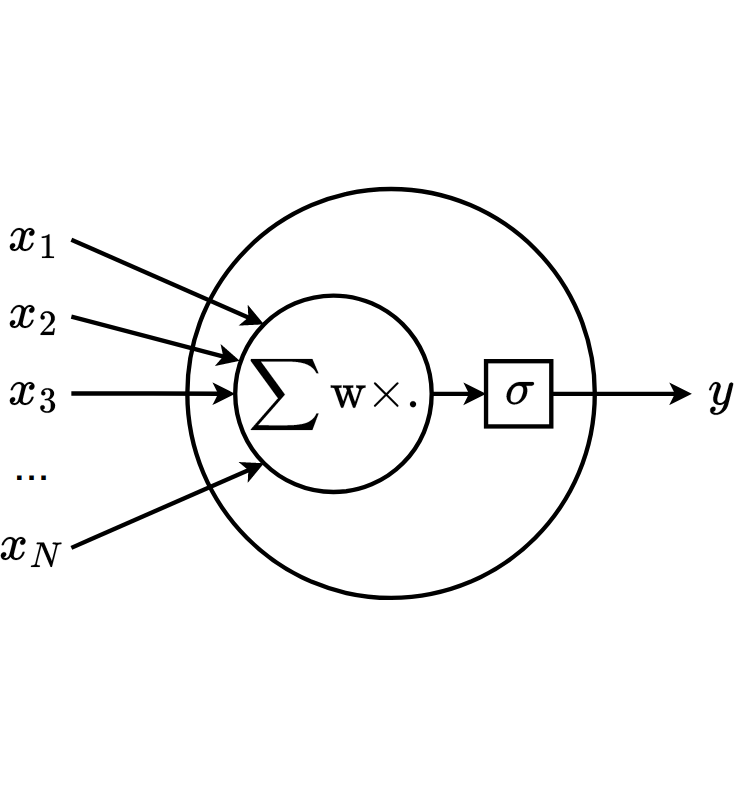
\includegraphics[width=\textwidth]{Figures/RL/perceptron.png}
        \caption{Perceptron}
        \label{fig:perceptron}
    \end{subfigure}
    \hfill
    \begin{subfigure}[b]{0.5\textwidth}
        \centering
        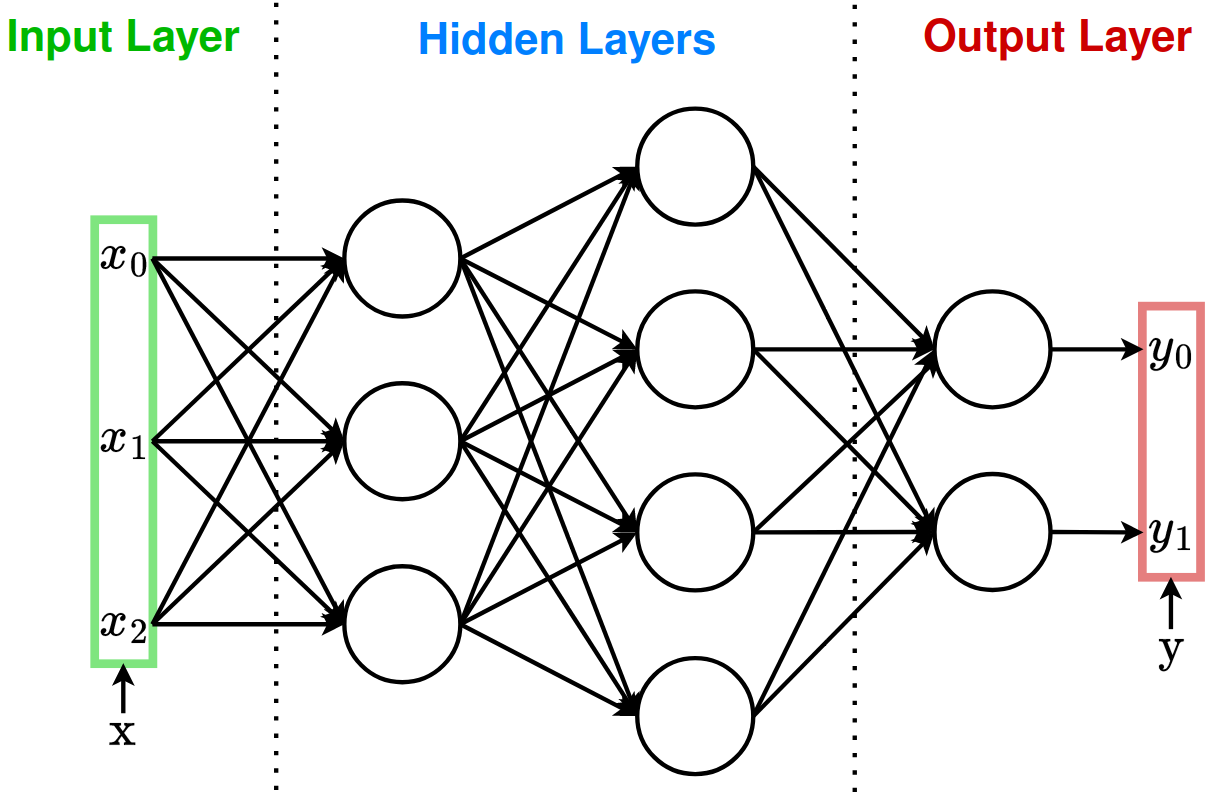
\includegraphics[width=\textwidth]{Figures/RL/mlp.png}
        \caption{Artificial neural network}
        \label{fig:mlp}
    \end{subfigure}
    \hfill
    \caption{Architecture of an artificial neural network (ANN). (a) The perceptron, i.e., the neuron-like element, transforming an input vector into a single output value. It does so with a summed vector multiplication with the neuron's weights $w$ and by using the activation function $\sigma$ that determines the activation of the neuron. (b) Example of ANN, with each circle representing a single perceptron. As there are more than one hidden layer, it is a multi-layer perceptron.}
    \label{fig:ann}
\end{figure}

% ANN
The term \textbf{artificial neural network} (ANN) designates a type of parameterised architecture that can be used to solve machine learning problems. Concretely, an ANN is a mathematical function that transforms the input vector, into an output vector of another form: $f:\mathbb{R}^N\rightarrow\mathbb{R}^M:f(x;\theta)=y$, with $x$ and $y$ respectively the input and output vectors of dimensions $N$ and $M$, and $\theta\in\mathbb{R}^{d^\theta}$ the vector of parameters of the neural network. The name "artificial neural network" comes from the actual form of this function. It can be decomposed into many simpler functions, each one of them acting as a neuron-like activation. The aggregation of multiple of these neurons in a computational graph builds the network architecture of the global function, as illustrated in Figure \ref{fig:mlp}.

% Perceptron
The neuron element of this network, illustrated in Figure \ref{fig:perceptron}, is called a \textbf{perceptron}~\citep{Rosenblatt1958_Perceptron}. It is a simple function that transforms a given input vector $x\in\mathbb{R}^N$ into a single output value $h(x;w)\in\mathbb{R}$ through a weighted sum. In this operation, each element of the input vector is multiplied by a learnable parameter $w_i\in\mathbb{R}$, also called a \textit{weight}, before being all summed together:
\begin{equation}
    h(x;w)=\sum_{i=1}^Nw_ix_i+b,
\end{equation}
with the input vector $x=\{x_i\}_{0<i\leq N}$, the weights $w=\{w_i\}_{0<i\leq N}$, and a bias parameter $b\in\mathbb{R}$. This bias, which is also a learnable parameter, is needed to learn more complex transformations. 

% Activation function
The result of this operation is then passed through an activation function $\sigma$ that determines the final output of the neuron:
\begin{equation}
    y=\sigma\left(h(x;w)\right)=\sigma\left(\sum_{i=1}^Nw_ix_i+b\right).
\end{equation}
This activation function is a non-linear transformation of the input. Without the non-linear activation, an aggregation of perceptrons could be rewritten as a linear transformation of the input. Thus, the purpose of $\sigma$ is to allow the neural network to model non-linear functions. Three examples of frequently used activation functions are the \textit{sigmoid} function, the hyperbolic tangent (\textit{Tanh}), and the Rectified Linear Unit (\textit{ReLU}; \cite{Glorot2011_ReLU}), all shown in Figure~\ref{fig:activ}.

% NN architecture & Parameters
Multiple perceptrons can be used to build a neural network, like in Figure \ref{fig:mlp}. In the classical ANN architecture, the neurons are structured in \textit{layers}. Each layer is composed of a fixed number of neurons, each neuron taking as input all the outputs of the previous layer. For this reason, this kind of layer is often called \textit{fully-connected}. Three distinct parts of the network are often identified: the input layer, the hidden layers, and the output layer. The input layer is made by the input vector. The output layer is the layer of neurons that will generate the output vector. Thus, both the dimensions of the input and output layers are determined by the required dimensions of the input and output vectors. On the other hand, between the input and output layers, the number of hidden layers and neurons in each one of them can be defined arbitrarily. Each neuron has its set of learnable parameters, whose dimension depends on the size of the last layer: one weight for each input, plus the bias. Thus, the parameters of the whole ANN, defined previously as $\theta$, is the set of all parameters (weights and biases) of all neurons in the network. 

% Activation functions
\begin{figure}
    \centering
    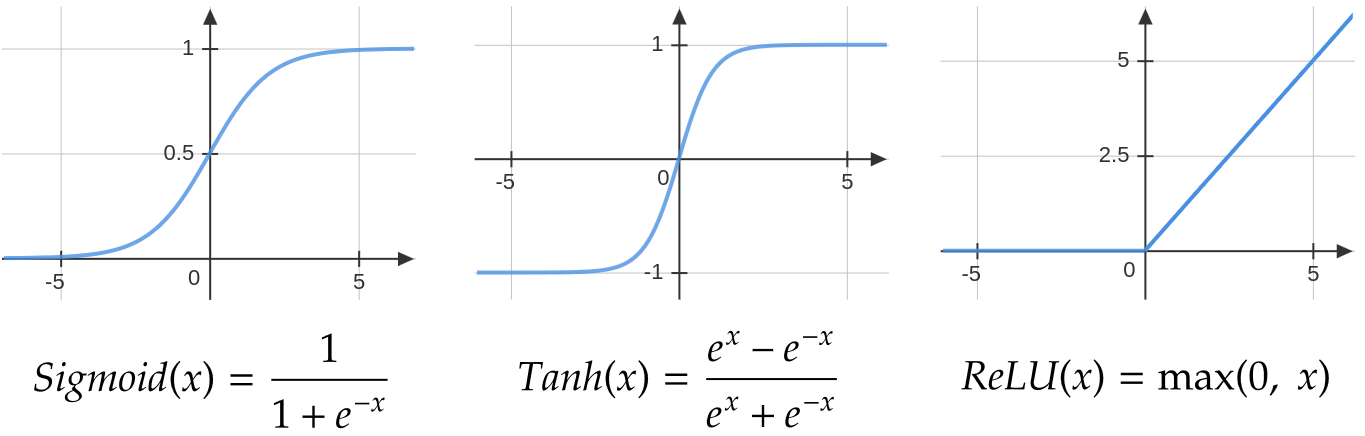
\includegraphics[width=0.9\textwidth]{Figures/RL/activ.png}
    \caption{Mathematical definitions and representations of three activation functions: sigmoid, hyperbolic tangent (Tanh), and rectified linear unit (ReLU).}
    \label{fig:activ}
\end{figure}

% Learning (gradient descent, forward/backward prop)
Learning these parameters can be done with gradient descent. When training the network, training examples $x$ are fed into the network, generating predicted outputs: $\widehat{y}=f(x;\theta)$. This is called the \textit{forward propagation}. The predictions are evaluated by a loss function that measures their quality with regard to the training objective. For example, in a supervised task, the objective of the model is to predict a target value $y$ associated with $x$ in the training data. In this case, the loss function measures the prediction error, which can be defined as the \textit{mean squared error}:
\begin{equation}
    L(\widehat{y};\theta)=\frac{1}{M}\sum_{i=1}^M(y_i-\widehat{y}_i)^2,
\end{equation}
with $M$ the dimension of the output layer. All operations made inside the network (i.e., $f$) are differentiable\footnote{The derivatives of some activation functions may not be defined everywhere (e.g., ReLU in 0), when that is the case, a value is arbitrarily defined for the missing derivatives (e.g., $\text{ReLU}'(0)=0$).}. This allows computing the gradient of the loss $L(\widehat{y};\theta)$ with regard to each parameter in the network, through a series of chain rules. Thus, the parameters can be updated to minimise the loss:
\begin{equation}
    \theta\leftarrow\theta-\alpha\nabla_\theta L(\theta),
\end{equation}
with a learning rate $\alpha\in]0,1]$. Notice the negative sign of the gradient used in gradient descent to minimise the loss, conversely to gradient ascent presented in Section \ref{sec:RL:Policy-based}, which was intended for maximising the RL objective. This process of going back to each parameter in the graph to compute its gradient and update it is often referred to as \textit{backward propagation}, or back-propagation.







\subsection{Recurrent Neural Networks}\label{sec:NN:RNN}

% RNN
The ANN architecture presented previously is one of many other more complex structures that specialise in particular tasks. One limitation of the ANN is that it struggles to handle sequential data, where inputs are arranged in time and can depend on previous inputs. For example, text is a form of sequential data where words and punctuation marks are arranged in a sequence. In this sequence, some words may have a strong correlation with others. In such cases, a neural network would benefit from learning these potential correlations by memorising some information from previous inputs. This is the idea behind \textbf{recurrent neural networks} (RNNs) that propose an architecture for handling sequential data, illustrated in Figure \ref{fig:rnn}. At each time step $t$, the RNN unit takes two inputs: the input data point $x_t\in\mathbb{R}^N$ and the hidden state of the last step $h_{t-1}\in\mathbb{R}^M$. The hidden state is a vector that carries information between each step of the process. At each step, it is updated with:
\begin{equation}
    h_t=\sigma\left(W_xx_t+W_hh_{t-1}+b\right),
\end{equation}
with $W_x\in\mathbb{R}^{N\times M}$ and $W_h\in\mathbb{R}^{M\times M}$ two matrices of learnable parameters, a bias vector $b\in\mathbb{R}^M$, and an activation function $\sigma$, which is often a Tanh in RNNs. The output is then a function of the hidden state: $y_t=g(h_t)$. Here, function $g$ can be a layer of perceptrons to output a vector in the required dimension. The RNN unit serves as a fundamental block that is often used inside a larger architecture. 

Notice that, all the computations made from the beginning of the sequence can be traced back in the final hidden state $h_T$ and written as a function of all inputs of the sequence: $h_T=g(x_T,h_{T-1})=g(x_T,g(x_{T-1},h_{T-2}))$, and so forth. Thus, as for the ANN, we can compute the gradients of a given loss function with regard to each parameter of the RNN unit. The specificity here is that the gradients are "back-propagated through time", as the loss at step $T$ depends on calculations done in all previous steps. This allows the RNN to learn the temporal correlation in the input sequences.

% Figure RNN
\begin{figure}
    \centering
    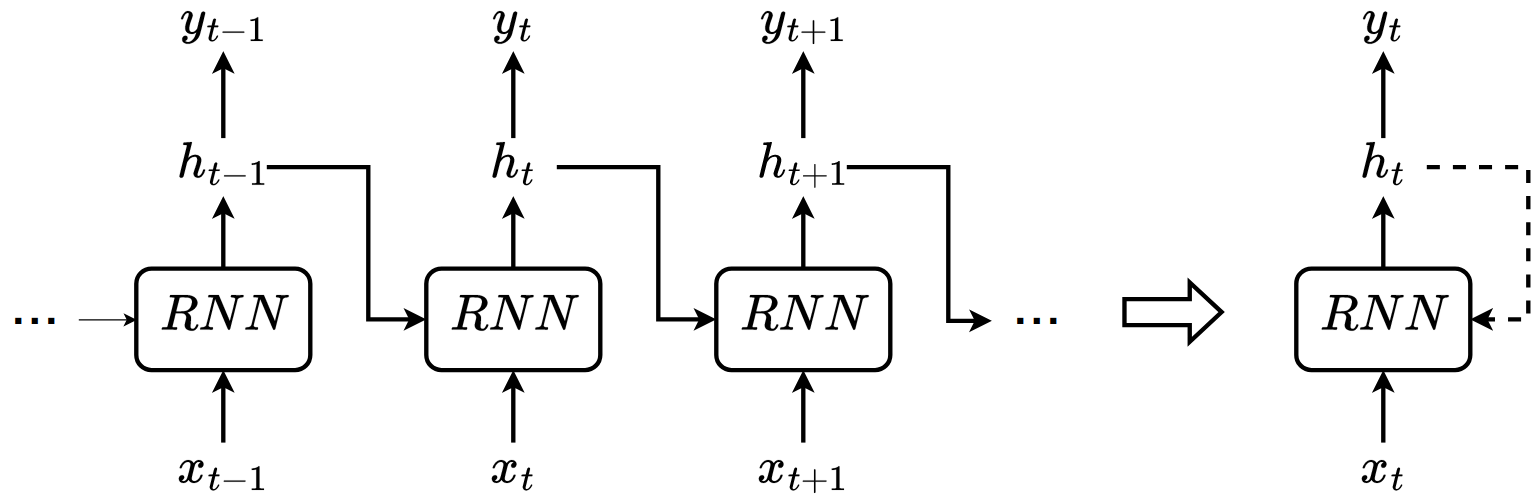
\includegraphics[width=0.8\textwidth]{Figures/RL/rnn.png}
    \caption{Illustration of a recurrent neural network (RNN) unit handling the sequence of inputs $x$. The left version shows the process unfolded in time, with the hidden state of step $t$ passed to the next step $t+1$. On the right is shown a condensed illustration of the RNN, with the dashed arrow indicating that $h_t$ is carried out to the next step.}
    \label{fig:rnn}
\end{figure}

% LSTM - GRU
While the hidden state of the RNN carries some information to the next step, in practice, this simple RNN struggles to memorise long-term information. In addition to that, it suffers from algorithmic flaws that prevent its use in many applications. However, better recurrent architectures have been developed to address these issues. The \textbf{Long Short-Term Memory} (LSTM) architecture~\citep{Hochreiter1997_LSTM} is one example (see Figure \ref{fig:lstm-gru}). Inside the LSTM unit, the information flows into various \textit{gates} that ensure the conservation or forgetting of some parts of the inputs. In addition to the hidden state, a "cell state" is also kept between steps. Intuitively, the cell state should carry more long-term memory than the hidden state. Another similar recurrent architecture is the \textbf{Gated Recurrent Unit} (GRU; \cite{Chung2014_GRU}). The GRU takes inspiration from the LSTM, but simplifies its architecture while keeping similar performance. In practice, both the LSTM and GRU are used in recent works to deal with sequential data. 

% Illustration LSTM et GRU
\begin{figure}
    \centering
    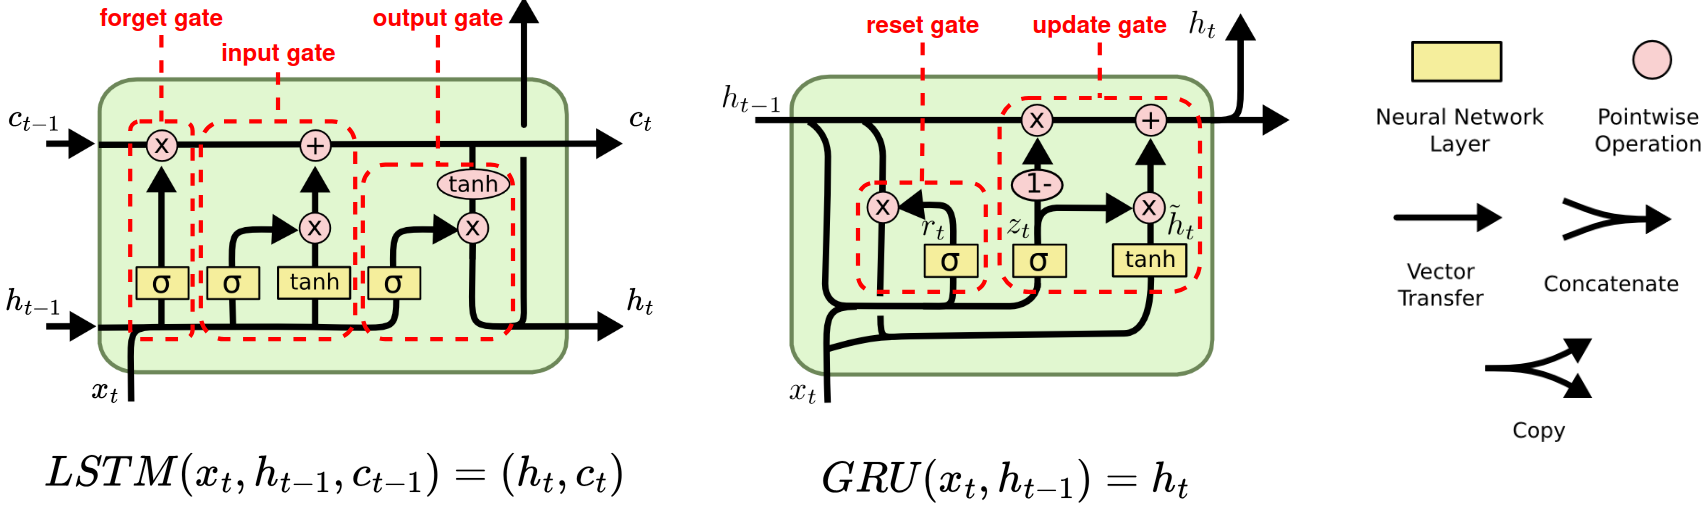
\includegraphics[width=0.9\textwidth]{Figures/RL/lstm-gru.png}
    \caption[LSTM-GRU]{Illustration of the Long Short-Term Memory (LSTM) and Gated Recurrent Unit (GRU) neural network architecture\footnotemark. Input information flows along the black arrows and passes through different "gates". These gates are neural networks that compute the outputs by updating the memory, forgetting some information and adding some new from the input $x_t$. In addition to the hidden state, the LSTM carries the cell state $c$ between each step to extend the memory capacities.}
    % PLACEHOLDER illustration, to do own
    \label{fig:lstm-gru}
\end{figure}

\footnotetext{Illustrations adapted from: \url{http://colah.github.io/posts/2015-08-Understanding-LSTMs/}.}

\subsection{Deep Neural Networks}\label{sec:NN:DeepLearning}

% Learning representations
The great strength of neural networks is their ability to automatically learn hidden relations in the training data. Take for example a computer vision task, where the objective is to determine the presence of a car in images. Classical machine learning algorithms usually require high-level features to solve such tasks: the presence of wheels in the picture, the number of such wheels, the presence of reflective material, and other common attributes of cars. With neural networks, such high-level features can be extracted automatically by looking at the training data. This is called \textit{representation learning}, where the neural network learns a set of weights (as described in Section \ref{sec:NN:ANN}) that produces accurate internal representations of the input data. Through careful training, the network learns how to understand the information given in the picture, to give an accurate prediction of the presence of a car. Because this is done automatically, this relieves the otherwise painful work of manually extracting and annotating important features in all training samples. This also allows the neural network to discover hidden features that could have been omitted in human-generated data (e.g., the fact that cars are often pictured on a road, so the presence of road signs might increase the probability of having a car in the image). However, there are also downsides to this. First, this automatic process of learning representations is done in a black box that is out of the control of human observers. The representation capacities of the neural network are embedded in the weights of the networks and are hard to understand and interpret. Second, these representation capacities still have a cost, now measured in the amount of training data at our disposal. To learn the complex relations in a very large space of input values and obtain good performance, neural networks usually require very large datasets of standardised data. Still, obtaining these datasets is often less difficult than manually extracting valuable features by hand. 

% MLP
It has been widely recognised that the number of layers in a neural network can greatly influence its performance in solving the task. In many cases, adding hidden layers can improve the representations learnt by the network. This can be understood intuitively by looking at each layer as a representation unit, where the first layer extracts low-level information, and subsequent layers each use the representation given by the last layer to extract more high-level features. This has led to the use of \textit{deep neural networks} that have more than one hidden layer, as in Figure \ref{fig:mlp}. These networks, often called \textbf{Multi-Layer Perceptrons} (MLPs), are the fundamental block of what is now called \textit{deep learning}, corresponding to any machine learning architecture that features deep neural networks.  

% Various Techniques and architectures (CNN, Attention, Transformers,...)
The MLP is the most basic form of deep neural architecture. It is often used to handle any input that can be represented as a vector. But, other architectures have been developed for specific types of inputs. For sequential data, the RNNs can be extended to have a deep architecture, with many recurrent units stacked on top of each other, as in Figure \ref{fig:deep-rnn}. For images, the \textbf{Convolutional Neural Networks} (CNNs; \cite{LeCun1989_CNN, Krizhevsky2012_AlexNet, Simonyan2015_VGG}) learn to detect complex patterns of pixel values that can then be used to recognise objects in images (see Figure \ref{fig:cnn}). Recently, the Transformer architecture~\citep{Vaswani2017_Transformer} have been introduced to handle sequential data, with better long-term memory than recurrent architectures. Transformers have been widely adopted in the machine learning community as a foundation for building better models. Extremely large Transformers with billions of learnable parameters have demonstrated superior performance in text generation~\citep{Ouyang2022_InstructGPT} and computer vision~\citep{Dosovitskiy2021_VisionTransformer}.

\begin{figure}
    \centering
    \hfill
    \begin{subfigure}[b]{0.3\textwidth}
        \centering
        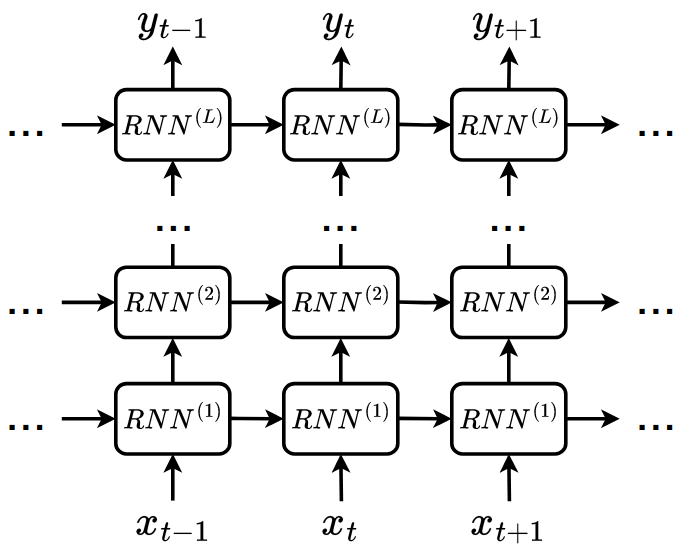
\includegraphics[width=\textwidth]{Figures/RL/deep-rnn.png}
        \caption{Deep RNN}
        \label{fig:deep-rnn}
    \end{subfigure}
    \hfill
    \begin{subfigure}[b]{0.6\textwidth}
        \centering
        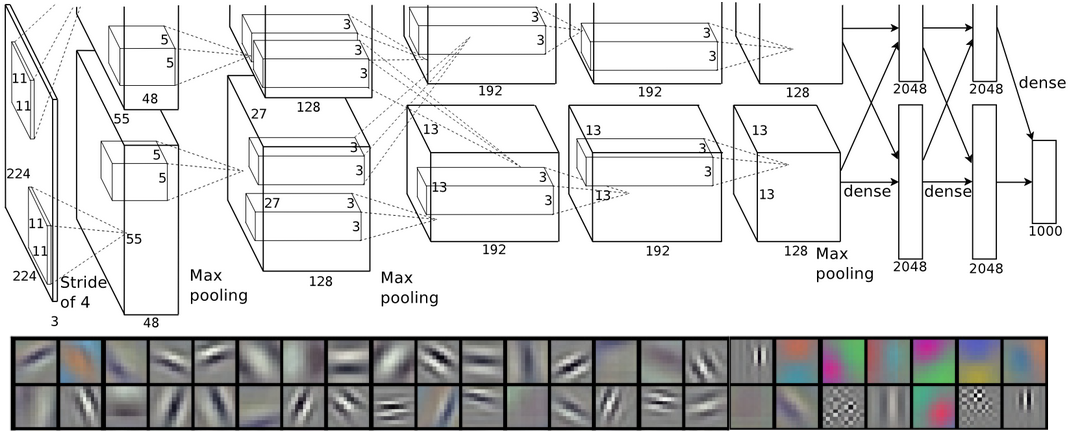
\includegraphics[width=\textwidth]{Figures/RL/vgg.png}
        \caption{Deep CNN}
        \label{fig:cnn}
    \end{subfigure}
    \hfill
    \caption{Two examples of deep neural network architectures. (a) A deep RNN, where the input $x_t$ passes through $L$ RNN units to compute the output $y_t$, with each unit passing its hidden state $h^{(i)}_t$ to the next layer $i+1$ and to the next step $t+1$. (b) Architecture of a deep convolutional network on top, and the bottom shows the learnt filters of the first convolutional layer that detect basic shapes in the images~\citep{Simonyan2015_VGG}.}
    \label{fig:ann}
\end{figure}

% Issues and hyperparameters
Overall, the impact of deep neural networks on machine learning has been tremendous. In the next section, we will see that deep learning is now a common technique in reinforcement learning research. But it also comes with its share of complications. First, training deep neural networks requires large amounts of data to train on. A larger neural network usually needs more data to train efficiently~\citep{Kaplan2020_ScalingLaws} and a common trend of greatly increasing model sizes to improve performance has been observed~\citep{Villalobos2022_ModelSizes}. Training larger models requires considerable computational power and access to computers equipped with Graphics Processing Units (GPUs) that can efficiently compute large matrix operations. This makes deep learning expensive and not accessible to anyone with a restricted budget. Even executing a trained model requires some computational capacities, which makes deployment on small platforms (e.g., robots) complicated. Lastly, deep neural networks are often complex and depend on many design choices to function well. They usually come with a long list of parameters, often called \textit{hyperparameters} to distinguish them from learnable parameters, that define their architecture and training setting: the number of layers, the dimension of the hidden layers, the learning rate, etc. Each one of these hyperparameters is a value that can impact the performance of the model and that needs to be tuned. But, despite these obstacles, deep learning is now widely used in artificial intelligence research and its applications, and is now a common building block of all state-of-the-art approaches in domains like computer vision and natural language processing.





% -------------------------------------------------------------------------




\section{Model-Free Deep Reinforcement Learning}\label{sec:DRL}

As in other branches of machine learning, deep learning has been a revolutionary technique for RL. It has enabled extending existing RL algorithms to operate in much more complex settings and has facilitated the development of new approaches for learning models, policies, and value functions. In this section, we will present the foundational works in model-free deep RL published in the last decade. These works form the basis for the majority of studies in both single-agent and multi-agent RL. While there is also significant research on model-based deep RL methods~\citep{Moerland2023_ModelRL}, we will not cover them here as they are not typically used in multi-agent settings and are thus outside the scope of this thesis. 


\subsection{Value-Based Methods}

\subsubsection{Deep Q-Learning}\label{sec:DRL:DQN}

% Motivations
In Section \ref{sec:RL:Qlearning}, we presented the Q-learning algorithm for learning a control policy using only an action-value function. We introduced the main limitations of this algorithm: scalability and generalisation. First, tabular Q-learning scales poorly to environments with large state-action spaces, as it needs to keep track of the learnt values of all state-action pairs. Second, Q-learning struggles to generalise its training knowledge to make good predictions in situations it has never experienced. It needs a thorough exploration of the environment to ensure that its predicted values are relevant. For these reasons, Q-learning is difficult to use in realistic settings where the number of possible states is large or infinite. 

These issues can be alleviated using a deep neural network in place of the value table. The \textbf{Deep Q-Network} (DQN), proposed by \cite{Mnih2013_DQN}, successfully adapts Q-learning to learn from visual data. To do so, it models the action-value as a CNN (see Section \ref{sec:NN:DeepLearning}) that takes as input frames from a video game and outputs the values of possible actions, as illustrated in Figure~\ref{fig:dqn}. Note that, while this first iteration of the DQN architecture uses a CNN, the term DQN is now used to describe any deep neural network architecture that computes action-values. 

The DQN is learnt completely end-to-end from the Q-learning objective. Concretely, the parameters of the network $\theta$ are optimised to minimise the following squared Bellman error:
\begin{equation}
    L(\theta)=\left(r_{t+1}+\gamma\max_{a}Q_{{\theta^-}}(s_{t+1},a)-Q_\theta(s_t,a_t)\right)^2,
\end{equation}
for any transition $\langle s_t,a_t,r_{t+1},s_{t+1}\rangle$ and with the discount factor $\gamma$. Notice the TD-target is computed using another network $Q_{\theta^-}$, named the \textit{target network}. The parameters $\theta^-$ are initialised as a copy of the main parameters $\theta$. Then, the target is fixed for a pre-defined number of training iterations, after which it is copied from the main network again, and so on. Using a slightly older, fixed version of $Q_\theta$ helps to stabilise training by giving a fixed target to aim for when minimising the Bellman error, instead of having it modified after each training iteration~\citep{Mnih2015_DQN}. 

% Experience replay
Another important feature of the DQN is its use of experience replay~\citep{Lin1992_ExperienceReplay}. Because deep Q-learning is off-policy, it can capitalise on all previously acquired experiences to train its deep neural network. The deep Q-learning algorithm thus alternates between acquiring experiences by interacting with the environment (typically executing the $\epsilon$-greedy policy), storing each experience in the replay buffer $\mathcal{B}$, and later training the DQN on a batch of samples randomly drawn from $\mathcal{B}$. Therefore, the DQN is trained to minimise the Mean Squared Bellman Error (MSBE) on the full batch:
\begin{equation}
    L(\theta)=\mathbb{E}_{\langle s,a,r,s'\rangle\sim\mathcal{B}}\left[\left(r+\gamma\max_{a'}Q_{{\theta^-}}(s',a')-Q_\theta(s,a)\right)^2\right].
    \label{eq:DQN}
\end{equation}
This batched loss is crucial for ensuring efficient training of a deep neural network. Plus, experience replay allows reusing each gathered experience multiple times and having more diverse batches, thus improving sample efficiency and avoiding overfitting the current policy.

DQN was the first successful instance of coupling RL with deep learning. It showed that deep RL was able to surpass human performance in video games, by learning only from visual data~\citep{Mnih2013_DQN}. It sparked a wave of research focused on using deep learning in existing RL algorithms and developing new learning methods specific to deep RL. 

\begin{figure}
    \centering
    \hfill
    \begin{subfigure}[b]{0.64\textwidth}
        \centering
        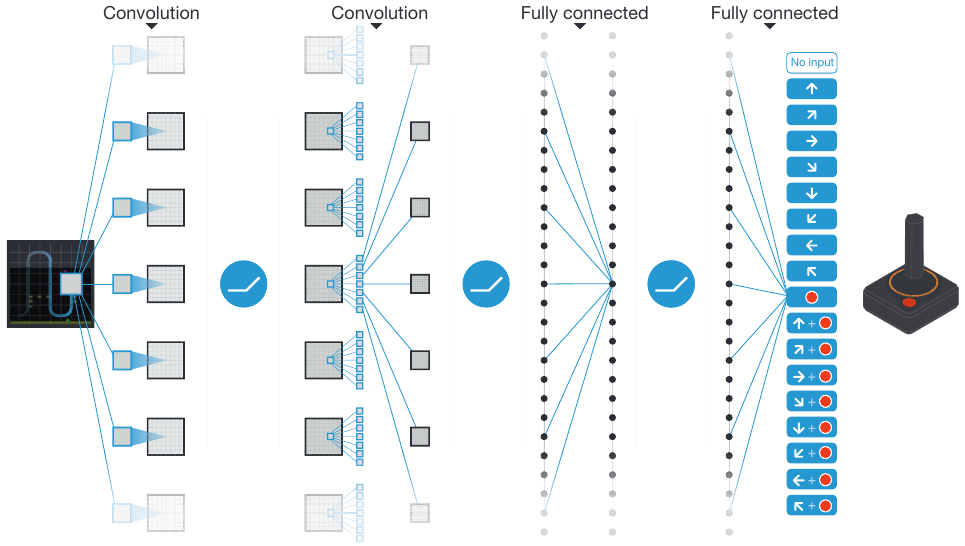
\includegraphics[width=\textwidth]{Figures/RL/dqn.png}
        \caption{Deep Q-Network}
        \label{fig:dqn}
    \end{subfigure}
    \hfill
    \begin{subfigure}[b]{0.35\textwidth}
        \centering
        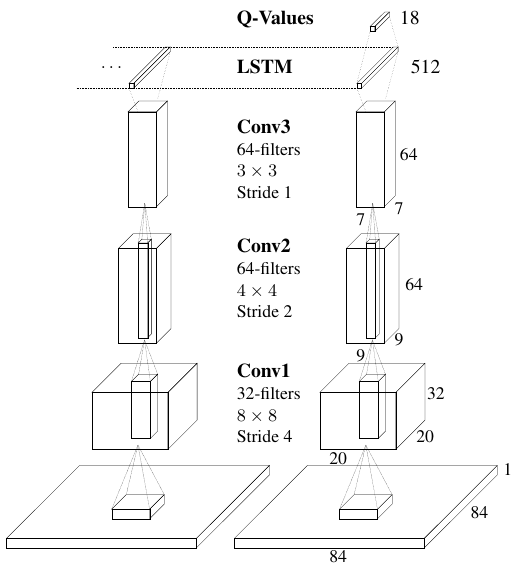
\includegraphics[width=\textwidth]{Figures/RL/drqn.png}
        \caption{Deep Recurrent Q-Network}
        \label{fig:drqn}
    \end{subfigure}
    \caption{DQN architectures. (a) The original DQN~\citep{Mnih2015_DQN}, with a series of convolution layers that analyse the input frame, followed by fully connected layers that output the value of each action. (b) Recurrent version of a DQN~\citep{Hausknecht2015_DRQN}, that adds an LSTM unit after the convolutions to allow some information to carry to future steps.}
    \label{fig:dqns}
\end{figure}



\subsubsection{DQN Extensions}\label{sec:DRL:Rainbow}

Following the introduction of the DQN, many works focused on improving this architecture using both old and new techniques. In their paper, \citet{Hessel2018_Rainbow} summarise the most important extensions and combine them into their method called \textit{Rainbow}. Some of these improvements concern the core functioning of the Q-learning algorithm:
\begin{itemize}
    \item \textit{Double Q-learning}~\citep{Hasselt2010_DoubleQlearning} modifies Equation~\ref{eq:DQN} to decouple the selection of the action to its evaluation when computing the Bellman error:
    \begin{equation}
        L(\theta)=\Bigl(r_{t+1}+\gamma Q_{{\theta^-}}(s_{t+1},\argmax_{a'}Q_\theta(s_{t+1},a'))-Q_\theta(s_t,a_t)\Bigl)^2.
        \label{eq:DDQN}
    \end{equation}
    In the TD-target, the action is selected by the main network $Q_\theta$ and evaluated by the target network $Q_{\theta^-}$. \citet{Hasselt2016_DoubleDQN} apply this idea to the DQN to improve its performance.

    \item The \textit{Dueling DQN}~\citep{Wang2016_DuelingDQN} proposes to decompose the action-value of an action $Q_(s,a)$ into two separate predictions: the value of the current state $V(s)$ and the \textit{advantage} of the action defined as $A(s,a)=Q(s,a)-V(s)$. They use a neural network architecture with two outputs, the state-value and advantage, which are then combined into the action-value. This allows them to learn a state-value and an action-value function in a single learning process with a deep Q-learning algorithm. 

    \item \textit{Distributional value learning}~\citep{Bellemare2017_DistributionalRL} proposes to learn a probability distribution over possible future returns, instead of learning to estimate the expected return of an action. Doing this allows to better account for multimodality in value distributions and generally improves learning stability. 
\end{itemize}
Other techniques focus on algorithmic and architectural improvements to DQN:
\begin{itemize}
    \item \textit{Prioritised experience replay}, proposed by \citet{Schaul2016_PER}, improves on experience replay by sampling experiences more often if they lead to bad value predictions (i.e., high Bellman errors) during training. This allows prioritising samples that the network fails to evaluate well, thus greatly improving sample efficiency. 

    \item \textit{Noisy DQN}~\citep{Fortunato2018_NoisyDQN} tackles the problem of exploration by adding noise to the parameters of the DQN. Note that \citet{Plappert2018_Noise} concurrently proposed a similar approach working with other deep RL algorithms. 
\end{itemize}
Rainbow shows that combining all these extensions greatly improves the performance and sample efficiency of DQN in a large variety of video games~\citep{Hessel2018_Rainbow}. 

\subsubsection{Deep Recurrent Q-Network}\label{sec:DRL:DRQN}

A remaining limitation of DQN is its lack of memory of previous events. This becomes a problem in partially observable environments where the agent does not get the full state of the environment, but rather a local observation describing its surroundings. In such settings, a memory-equipped agent could explore its surroundings to build a better understanding of the current state of the environment. To achieve this, \citet{Hausknecht2015_DRQN} augment the DQN architecture with an LSTM unit (see Section \ref{sec:NN:RNN}) to learn to memorise important information for future steps (see Figure~\ref{fig:drqn}). They show that this makes agents more robust to losses in their observations. This approach has been combined with distributed training by \citet{Kapturowski2018_R2D2}, largely surpassing previous works on some Atari games. As we will see in Chapter \ref{ChapterMADRL}, using recurrent units has been widely adopted in multi-agent deep RL to deal with partial information given to each agent. 





\subsection{Policy-Based Methods}\label{sec:DRL:Policy}

\subsubsection{Deep Deterministic Policy Gradient}\label{sec:DRL:DDPG}

% DDPG
In Section \ref{sec:Policy:Actor-Critic}, we introduced the actor-critic architecture that combines a policy (i.e., actor) and a value (i.e., critic) to open up the possibilities of RL training. Following the introduction of the DQN, similar ideas were implemented to extend actor-critics with deep learning. The \textbf{Deep Deterministic Policy Gradient} (DDPG; \cite{Lillicrap2015_DDPG}) was proposed to extend the DQN to work with continuous actions. Like in the original DPG (see Section \ref{sec:Policy:Actor-Critic}), a deterministic policy function $\pi_\theta$ is learnt to select actions in a continuous space and an action-value function $Q_\phi$ is used to predict the quality of the selected actions. Here, both of these are modelled using deep neural networks. As in Double Q-learning (see Section \ref{sec:DRL:Rainbow}), both the policy and value functions are doubled with target functions $\pi_{\theta^-}$ and $Q_{\phi^-}$, respectively. The targets are used to compute the TD-target for computing the MSBE loss:
\begin{equation}
    L(\Theta)=\mathbb{E}_{\langle s,a,r,s'\rangle\sim\mathcal{B}}\left[\left(r+\gamma Q_{\phi^-}(s',\pi_{\theta^-}(s'))-Q_\phi(s,a)\right)^2\right].
    \label{eq:DDPG}
\end{equation}
The target parameters $\Theta^-=\{\theta^-,\phi^-\}$ are initialised as copies of the main parameters $\Theta$ and later slowly moved towards the main networks with a "soft" update: $\Theta^-\leftarrow\tau\Theta^-+(1-\tau)\Theta$, with $0<\tau\ll1$. Using this approach, combined with experience replay and other small tricks, DDPG managed to greatly improve on the non-deep DPG. 

% TD3
\citet{Fujimoto2018_TD3} pointed out that DDPG, as all Q-learning methods, suffers from an overestimation of action-values induced by using a bad value estimate for computing the optimisation objective. While Double Q-learning helps address this issue, it does not completely solve it. They propose an extension of DDPG, named \textit{Twin Delayed DDPG} (TD3), that better mitigates the overestimation problem with three tricks:
\begin{itemize}
    \item First (\textit{Twin}), TD3 learns two action-value functions instead of one and uses the smaller values of the two when computing the TD-target. 
    \item Second (\textit{Delayed}), the policy function is trained less often than the action-value functions (one policy update for every two value updates) to make the policy less prone to value errors. 
    \item Third, the value estimates are smoothed by adding a small clipped noise on the target policy actions when computing the TD-target. This prevents having high spikes of value on some particular actions that the deterministic policy would then overfit to.
\end{itemize}
Therefore, TD3 computes the TD-target by taking the minimum value given by the twin DQNs and adding the clipped noise to the policy's action:
\begin{gather}
    y(r,s')=r+\gamma\min_{i=1,2}Q_{\phi_i^-}(s',\pi_{\theta^-}(s')+\epsilon), \\
    \epsilon\sim\text{clip}(\mathcal{N}(0,\sigma),-c,c),
\end{gather}
for some transition $\langle s,a,r,s'\rangle$, with hyperparameters $\sigma$ and $c$ controlling the width of the smoothing noise. The twin DQNs are both trained to minimise their MSBE:
\begin{equation}
    L(\phi_i)=\mathbb{E}_{\langle s,a,r,s'\rangle\sim\mathcal{B}}\left[\left(y(r,s')-Q_{\phi_i}(s,a)\right)^2\right], \text{ with } i\in\{1,2\}.
\end{equation}
These modifications are shown to improve the stability and performance of DDPG.


% \subsubsection{Asynchronous Advantage Actor Critics}

\subsubsection{Trust Region Policy Updates}\label{sec:DRL:PPO}

% Policy gradient limitations
In Section~\ref{sec:Policy:PolicyGradientTheorem}, we presented the policy gradient method used in most policy-based algorithms, which aims at maximising the following objective for learning a stochastic policy:
\begin{equation}
    L^{PG}(\theta)=\mathbb{E}_\pi\left[\log\pi_\theta(a|s)Q_{\pi_\theta}(s,a)\right].\footnote{If we compute the gradient of this objective, we find the formulation of Equation~\ref{eq:PolicyGradient:sampleA} as, by chain rule, $\nabla_x\log f(x)=\frac{\nabla_xf(x)}{f(x)}$.}
\end{equation}
This objective has two important limitations. First, the size of the learning step is difficult to define. In the context of learning a policy that generates the data it is trained on, a too big learning step could be catastrophic if it engenders a bad policy. In supervised learning, a bad learning step can be recovered later because the training data is still good. Here, a bad policy would change the distribution of samples and could then be very hard to recover from. Second, this objective theoretically limits the algorithm to use each gathered experience only one time (\cite{Schulman2017_PPO} shows doing multiple updates damages performance), which makes policy gradient algorithms less sample efficient. 

% TRPO
% propose new objective with pi_old, good estimate of PG if pi_old is close to pi
% constraint on KLdiv to ensure that pi doesn't go too far from pi_old
% minimax objective
\citet{Schulman2015_TRPO} propose to modify the policy gradient objective to tackle these issues. The objective is replaced by the following surrogate objective:
\begin{equation}
    L^{surr}(\theta)=\mathbb{E}_{\pi_\theta}\left[\frac{\pi_\theta(a|s)}{\pi_{\theta_{old}}(a|s)}A_{\pi_\theta}(s,a)\right],
    \label{eq:DRL:TRPO-surr}
\end{equation}
where $\pi_{\theta_{old}}$ is another policy and $A_{\pi_\theta}$ is the advantage function defined as $A_\pi(s,a)=Q_\pi(s,a)-V_\pi(s)$~\citep{Baird1995_ResidAlgs}. Using the advantage is equivalent to the action-value but reduces the variance of the value estimate. This objective is shown to be a good approximation of the policy gradient one, only if $\pi_{\theta_{old}}$ is close to $\pi_\theta$. Thus, for this to work, a constraint must be added to ensure that $\pi_\theta$ does not diverge too much from the old version:
\begin{equation}
    \mathbb{E}_{\pi_\theta}\left[KL(\pi_{\theta_{old}}(\cdot|s),\pi_\theta(\cdot|s))\right]\leq\delta,
    \label{eq:DRL:TRPO-constraint}
\end{equation}
with $KL$ measuring the Kullback-Leibler divergence between the two distributions and $\delta$ a hyperparameter for controlling the amount of allowed divergence. Maximising $L^{surr}$ while respecting the constraint of (\ref{eq:DRL:TRPO-constraint}) ensures that the update stays in a "trust region". The resulting \textbf{Trust Region Policy Optimisation} (TRPO) algorithm can do multiple updates on one sampled experience, with $\pi_{\theta_{old}}$ being the policy used when gathering the experience, to improve $\pi_\theta$ as much as possible for each interaction with the environment.

% PPO (... many update per sample), 
% ?Intuitive idea of ppo (going in the direction of good updates)
% improvements on PPO and implementations tricks
While the approach TRPO has great advantages, its implementation is difficult, mainly because of the constraint on KL divergence second-order optimisation. To simplify this, \textbf{Proximal Policy Optimisation} (PPO; \cite{Schulman2017_PPO}) removes the constraint and instead clips the objective to limit the magnitude of the updates. The new, clipped objective is defined as follows:
\begin{equation}
    L^{clip}(\theta)=\mathbb{E}_{\pi_\theta}\left[\min(r(\theta)A_{\pi_\theta}(s,a),\text{clip}(r(\theta),1-\epsilon,1+\epsilon)A_{\pi_\theta}(s,a)\right],
    \label{eq:PPO-objective}
\end{equation}
with $r(\theta)$ the probability ratio from TRPO, $r(\theta)=\frac{\pi_\theta(a|s)}{\pi_{\theta_{old}}(a|s)}$, and $\epsilon$ a hyperparameter typically close to 0. This objective first clips the ratio to be close to 1 to ensure that the new policy does not diverge too much from the old one. Then, they take the minimum of the clipped and unclipped objectives to make a lower bound of the unclipped objective. This objective is simpler to compute and optimise, making PPO simpler to implement. The full objective maximised by PPO is the following:
\begin{equation}
    L^{PPO}(\theta,\phi)=\mathbb{E}_{\pi_\theta}\left[L^{clip}(\theta)-c_1L^{VF}(\phi)+c_2H(\pi_\theta)\right]
    \label{eq:PPOloss}
\end{equation}
where $c_1$ and $c_2$ are coefficients for the two secondary losses. $L^{VF}$ is the MSBE loss for learning the value function used to compute the advantage in (\ref{eq:PPO-objective}), using a technique called Generalised Advantage Estimation~\citep{Schulman2016_GAE}. The third term uses the entropy of the policy, defined as $H(\pi)=\mathbb{E}_\pi[-\log\pi(a|s)]$, to induce exploration. Maximising entropy means increasing the randomness of the policy. This bonus ensures random exploration of new policies. The main objective $L^{clip}$ evaluates each modification with regard to expected future returns. 

PPO is considered one of, if not the best existing deep RL algorithm. It has been deeply studied and improved in various ways since its first release. Many implementation tricks have been identified to be crucial to the performance of the algorithm~\citep{Hendersion2018_Matters, Engstrom2020_PPOImplement}. 



\subsubsection{Soft Actor-Critic}\label{sec:DRL:SAC}

% combine maximum entropy & soft q learning
Finally, we present the Soft Actor-Critic (SAC) algorithm~\citep{Haarnoja2018_SAC} that tackles the poor sample efficiency of on-policy algorithms and the brittleness of off-policy algorithms with regard to their hyperparameters. To do so, it builds an off-policy actor-critic algorithm with a stochastic policy and a "soft" action-value function. The policy is trained on samples drawn from the replay memory $\mathcal{B}$ to maximise the expected future rewards and an entropy bonus for exploration, as in PPO:
\begin{equation}
    L^\pi(\theta)=\mathbb{E}_{s\sim\mathcal{B},a\sim\pi_\theta}\left[Q_\phi(s,a)+\alpha H(\pi_\theta)\right],
\end{equation}
with $alpha$ controlling the importance of the entropy bonus. As in DDPG, the action is sampled from the policy and evaluated by the value function. Maximising this objective operates a trade-off between generating actions with high action-values and inducing diverse behaviours. 

To learn the action-value function, the authors take inspiration from soft Q-learning~\citep{Haarnoja2017_SoftQLearning}, where entropy maximisation is included in the value learning algorithm. The soft action-value is trained to minimise the soft MSBE for any transition drawn from the buffer:
\begin{equation}
    L^Q(\phi)=\mathbb{E}_{\langle s,a,r,s'\rangle\sim\mathcal{B}}\left[\frac{1}{2}\big(Q_\phi(s_t,a_t)-y^{soft}(r,s')\big)^2\right],
\end{equation}
where
\begin{equation}
    y^{soft}(r,s')=r+\gamma\mathbb{E}_{a'\sim\pi_\theta}[Q_\phi(s',a')-\alpha\log\pi_\theta(a'|s')].
\end{equation}
The target in this objective also has a bonus on the entropy of the policy, which makes the action-value function favour actions where the policy is uncertain. They show that this use of entropy maximisation with a stochastic policy greatly improves the stability and robustness of their algorithm. 



% \subsection{Model-based methods}\label{sec:DRL:Model}

% \subsubsection{Planning with Deep RL}\label{sec:DRL:Planning}

% \subsubsection{World models}\label{sec:DRL:WorldModels}





% -------------------------------------------------------------------------

% Conclusion du chapitre (?)
% "on a pas parlé de tout mais présenté les tehcniques qu'on utilise et le domaine du RL dans lequel on se situe"

\section{Conclusion}

In this chapter, we have presented the field of reinforcement learning for training a single agent to solve tasks from its own experience. Understanding the different techniques behind reinforcement learning algorithms is important to understand the challenges we will face later: \textit{how having multiple agents will impact learning} and \textit{how we can use and shape these learning algorithms to fit the requirements of robotic settings}. In the next chapters, we will investigate these issues and propose new approaches for tackling them. 